% Terry Tao, on writing: https://terrytao.wordpress.com/advice-on-writing-papers/
% https://terrytao.wordpress.com/2007/03/18/why-global-regularity-for-navier-stokes-is-hard/#comment-625243


% https://fenicsproject.org/olddocs/dolfin/1.5.0/python/demo/documented/stokes-iterative/python/documentation.html
%
%
%
%
%

% \documentclass{article}
\documentclass[11pt,a4paper]{memoir}
% \setsecnumdepth{subsubsection}
\setsecnumdepth{subsection}
\setcounter{tocdepth}{2}
\setlrmarginsandblock{3cm}{3cm}{*} % Centre adjustment
\setulmarginsandblock{2.5cm}{*}{1}
\checkandfixthelayout 

\usepackage{amsmath}
\usepackage{amssymb}
\usepackage{mathtools}
\usepackage{microtype}
\usepackage{dirtytalk}
\usepackage{relsize}
\usepackage{csquotes}
\usepackage{epigraph}
\usepackage{physics}
\usepackage{cancel}
\usepackage{bm}
\newcommand{\bb}{\begin{bmatrix}}
\newcommand{\bbe}{\end{bmatrix}}
\newcommand{\pr}{\prime}
\newcommand{\ppr}{{\prime\prime}}
\newcommand{\pppr}{{\prime\prime\prime}}
\newcommand{\inner}[1]{\left<#1\right>}
\newcommand{\fancyA}{\mathcal{A}}
\newcommand{\fancyL}{\mathcal{L}}
\newcommand{\fancyN}{\mathcal{N}}
\newcommand{\fancyP}{\mathcal{P}}
% \newcommand{\norm}[1]{\left\Vert#1\right\Vert}
\newcommand{\om}{{\Omega}}
\newcommand{\pom}{{\partial\Omega}}
\newcommand{\omn}{{\Omega_0}}
\newcommand{\pomn}{{\partial\Omega_0}}
\newcommand{\diver}{\text{div}}
\newcommand{\Part}[2]{\frac{\partial #1}{\partial #2}}
% footnotes
\renewcommand\footnoterule{}

\newcommand{\todo}[1]{\vskip 0.1in \hrule \vskip 0.03in {#1} \vskip 0.03in \hrule \vskip 0.1in}

\begin{document}
\title{\Huge \textbf{The finite element method for the Navier-Stokes equations}}
\author{Lucas Payne}

\maketitle

\tableofcontents

\chapter{Mechanics}
\chapterprecishere{
Corpus omne perseverare in statu suo quiescendi vel movendi uniformiter in directum, nisi quatenus a viribus impressis cogitur statum suum mutare.
\\\\
Mutationem motus proportionalem esse vi motrici impressae, \& fieri secundum lineam rectam qua vis illa imprimitur.
\\\\
Actioni contrariam semper \& aequalem esse reactionem: sive corporum duorum actiones in se mutuo semper esse aequales \& in partes contrarias dirigi.
\par\raggedleft \textup{Newton \cite{newton}}}
% \section{Newton's laws of motion} % <<<
% 
% Newton's three laws, namely those of inertia, force, and equilibrium, have found universal success in application
% to mechanical systems such as the pendulum, the motion of a rigid body, the evolution of a bending beam, and, as we shall see,
% the motion of a fluid. \textit{Mechanics} could be thought of as the study of physical motion, but the word ``physical'' might be misleading.
% Newton's principles are mathematical in nature, applicable to the study of motion in a general sense as some unambiguously
% measurable state which evolves in time.
% 
% \subsection{Symmetry, momenta, and inertia}
% Mechanics as a theory of physical motion will require a definition of physical motion. A first attempt might be to posit
% that ``physical states'' are representable as points in a finite-dimensional manifold, which we call the configuration space $C$, which is the case for typical
% notions of state such as the two angles in a double pendulum, or the position and orientation of a rigid body. We might define a motion as
% a continuous time-parameterised curve
%     $$\gamma: [t_1, t_2] \rightarrow C.$$
% 
% % (--- motivation of $F = ma$, and momenta as fundamental quantity).
% 
% We start in the middle:
% \begin{equation}
%     \text{Total force = change of momentum}.
% \end{equation}
% In this form, Newton's second law of motion states that a (non-explanatory) measurement of change of momentum will be called ``force''.
% 
% 
% 
% % >>>
% \section{The Euler-Lagrange equations: \small{From $F = ma$ to $\Part{\fancyL}{q} - \frac{d}{dt}\Part{\fancyL}{\dot{q}} = 0$}} % <<<
% \subsection{A Lagrangian of a mechanical system}
% Force is an intensive measurement of the change in momentum. In the language of calculus,
% \begin{equation}\label{force_equation}
%     \int_{s_1}^{s_2} F\,dt = \fancyP(s_2) - \fancyP(s_1)
% \end{equation}
% for all time subintervals $[s_1, s_2] \subset [t_1, t_2]$. If we restrict $F$ to be conservative and a function only of position $q$, then we may
% let $F = -\Part{V}{q}$ for some potential function $V$. Suppose also that $\mathcal{P} = \Part{T}{\dot{q}}$ for some potential function
% (called the ``kinetic energy'') independent
% of position $q$. We then define a Lagrangian of the mechanical system to be
%     $$\fancyL(q, \dot{q}, t) = T(\dot{q}, t) - V(q, t) = \text{kinetic} - \text{potential}.$$
% By definition, we have the force equation \eqref{force_equation} as
%     $$-\int_{s_1}^{s_2} \Part{\fancyL}{q}\,dt = \Part{\fancyL}{\dot{q}}(s_2) - \Part{\fancyL}{\dot{q}}(s_1).$$
% The step toward the calculus of variations (---)
% \begin{equation}\label{el_inner_product_sum}
%         \int_{s_1}^{s_2} \Part{\fancyL}{q}h\,dt + \int_{s_1}^{s_2} \Part{\fancyL}{\dot{q}}\frac{dh}{dt}\,dt = 0
%     \quad\equiv\quad    \left<\Part{\fancyL}{q}, h\right> + \left<\Part{\fancyL}{\dot{q}}, \frac{dh}{dt}\right> = 0.
% \end{equation}
% Adjointness of differential operator $\frac{d}{dt}$ to $-\frac{d}{dt}$, and integration by parts. (---)
% By linearity, we then get the reformulation of \eqref{el_inner_product_sum} as
% \newcommand{\gateauxlagrangian}{\Part{\fancyL}{q} - \frac{d}{dt}\Part{\fancyL}{\dot{q}}}
%     $$\left<\gateauxlagrangian, h\right> = 0$$
% for all perturbation functions $h$.
% 
% \subsection{The first variation of a functional}
% In the calculus of variations, $\gateauxlagrangian$ is an instance of the \textit{G\^ateaux derivative}, also called the ``first variation'' of
% the functional
% \begin{align*}
%     S[q] \coloneqq \int_{t_1}^{t_2} \fancyL(q, \dot{q}, t)\,dt.
% \end{align*}
% The first variation measures response of the value of $S$, called the \textit{action}, to perturbations of the (differentiable) input function $q$,
% and is denoted
% \begin{equation}
%     \frac{\delta S}{\delta q(t)} \coloneqq \gateauxlagrangian.
% \end{equation}
% The first variation is linear in the perturbation function, and so another term for the G\^ateaux derivative could be ``functional gradient''.
% Setting this to zero gives the Euler-Lagrange equations, and the practice of determining trajectories of motions as stationary curves of the action is called the ``principle of stationary action''.
% 
% \subsection{From the Lagrangian to the equations of motion}
% In the framework of Lagrangian mechanics, $\fancyP \coloneqq \Part{\fancyL}{\dot{q}}$ is the momentum. If there are $d$ degrees of freedom
% in the mechanical system, and we suppose that $q_1,\cdots,q_d$ are (local) variables of state, then we say that $\fancyP_i \coloneqq \Part{\fancyL}{\dot{q}_i}$
% are \textit{conjugate} to the $q_i$.
% 
% (---) By inducing the equations of motion by a Lagrangian, we get systems with a ``physical interpretation'' with ``physically meaningful'' force measurements.
% 
% \subsection{Why ---?}
% These variational ideas appear because, no matter if our configuration space is finite-dimensional, time forms a continuum, and therefore if we
% globally consider the calculus of the motion as a whole, it must be a ``variational'' calculus. (---)
% 
% (---) Physical process, conservation laws, conservative forces (hint at thermodynamics limiting the range of stress tensors?)
% 
% When we consider mechanical models of continuum processes, we will see that these same ideas appear in the spatial dimensions too.
% A variational understanding of a continuum mechanics model leads very easily to a class of methods called Galerkin methods for solving
% the corresponding (PDE) equations of motion.
% 
% 
% % >>>

The calculus of variations.

\chapter{Continuum mechanics}
\section{Introduction}
--- Introduction.

Although the focus later will be on fluid mechanics, a large set of fundamental concepts of solid and fluid mechanics
are the same. The key distinction appears when one focuses on displacements and materials with ``shear strength'' (solids)  versus flows
and materials with no shear strength (common fluids).

\section{Transport} % <<<

Before considering continuum processes in the framework of Newtonian and Lagrangian mechanics, we will look at a fundamental notion of a ``motion''
of a point in a function space. Many continuum models in physics, such as the heat equation,
Maxwell's equations, and the equations of fluid motion, are formed by \textit{conservation equations}. These laws posit that the
evolution of the state (represented by a function) is
due to the transport of the quantity that the function measures, which is either pushed around (by some flux either predetermined or dependent on the current state)
or created and destroyed at sources and sinks.

% (figure of some manifold embedded in space, and some vector field pushing quantity around)
\begin{center}
\includegraphics[angle=90,page=11,width=0.56\linewidth]{figures/2.pdf}
\end{center}

We consider here the transport of quantities (scalar, vector, and tensor) on a general finite-dimensional manifold $M$,
colloquially called ``the continuum''. All transporting vector fields (or flux functions) are considered to be tangent to this manifold $M$.

\subsection{Continuity equations and conservation laws}\label{conservation_laws}
\subsubsection{The integral form of a continuity equation}
Consider some spatial quantity $\phi$ on $M$ and a flux function $j$ which by which
this quantity flows around $M$. For clarity, we will begin by specializing $\phi$ to be a scalar, although later we will find it useful to
transport vector quantities such as momentum. By definition we want this flux function to just push quantity around, and not create or destroy it:
the creation and destruction of quantity is determined by some arbitrary source function $s$ (of the same kind as $\phi$). These variables are related by the
conservation condition
\begin{equation}\label{continuity_equation}
    \frac{d}{dt} \int_{\Omega_0} \phi\,dx = \int_{\Omega_0} s\,dx + \int_{\pomn} \phi j \cdot \left(-\hat{n}\right)\,dx
\end{equation}
for arbitrary control volumes $\Omega_0$ in the continuum. The term $-\hat{n}$ denotes the inward-pointing normal to the boundary of the control volume. This simply says that the change in the total quantity in the fixed control volume is accounted for exactly by that quantity pushed through the boundary by the flux function $j$, and the internal sources and sinks of quantity $s$.
% --- $s_B$ as a boundary term? Why introduce this? Seems to be needed for the derivation of surface forces.
% (--- It may be useful to add $s_G$ as a boundary source term at $\pomn \cap \pom$ so Dirac delta ideas don't need to be used for non-fluxed boundary source (or, for example, the domain might be a subdomain where the transported function is unknown outside, so the term is introduced through $s_G$.))

\subsubsection{The differential form of a continuity equation}
A common technique in continuum modelling is the use of Stokes' theorem to simplify integral expressions.
Equation \eqref{continuity_equation} becomes
\begin{equation}\label{continuity_equation_differential}
    \Part{\phi}{t} = s - \nabla\cdot (\phi j)
\end{equation}
assuming that $\phi j$ is sufficiently differentiable such that the limiting integral exists.
It should be noted that Stokes' theorem and its specialisations are really \textit{definitions} of pointwise quantities
such as the divergence and curl as limits of these integral expressions for arbitrarily small regions.
Continuity relations are most naturally expressed in form \eqref{continuity_equation}, while the form
\eqref{continuity_equation_differential} may be more useful for techniques such as finite differences.
For example, it is a theorem of Gauss that in Euclidean space ($M = \mathbb{R}^3$) we have
\begin{equation}\label{gauss_euclidean_divergence}
    \nabla \cdot j = \Part{j_x}{x} + \Part{j_y}{y} + \Part{j_z}{z},
\end{equation}
and we get \eqref{continuity_equation_differential} in the form
\begin{equation}\label{continuity_equation_expanded}
    \Part{\phi}{t} = s - \nabla \phi \cdot j - \phi\left(\Part{j_x}{x} + \Part{j_y}{y} + \Part{j_z}{z}\right),
\end{equation}
by the product rule.
As one equation in a system of PDEs, \eqref{continuity_equation_expanded} is readily discretised by finite differences. For example, using forward difference in time and
central differences in space, our discrete scheme is
\begin{equation}\label{continuity_equation_finite_differences}
\begin{split}
    \frac{\phi(t + \Delta t) - \phi(t)}{\Delta t} = s &-\frac{\phi(\hat{x} + e_1\Delta x/2) - \phi(\hat{x} - e_1\Delta x/2)}{\Delta x}j_x \\
                                                      &-\frac{\phi(\hat{x} + e_2\Delta y/2) - \phi(\hat{x} - e_2\Delta y/2)}{\Delta y}j_y \\
                                                      &-\frac{\phi(\hat{x} + e_3\Delta z/2) - \phi(\hat{x} - e_3\Delta z/2)}{\Delta z}j_z \\
                                                      &-\frac{j_x(\hat{x} + e_1\Delta x/2) - j_x(\hat{x} - e_1\Delta x/2)}{\Delta x}\phi \\
                                                      &-\frac{j_y(\hat{x} + e_2\Delta y/2) - j_y(\hat{x} - e_2\Delta y/2)}{\Delta y}\phi \\
                                                      &-\frac{j_z(\hat{x} + e_3\Delta z/2) - j_z(\hat{x} - e_3\Delta z/2)}{\Delta z}\phi
\end{split}
\end{equation}
for $e_1,e_2,e_3$ the standard basis vectors in $\mathbb{R}^3$.
Later, when we discuss numerical methods for solving continuum models, we will not take this route. The methods of interest, \textit{Galerkin} methods,
work naturally with the integral form \eqref{continuity_equation}.
It will be seen later that some constructions in the presentation of Galerkin methods, such as the ``weak form'' of a PDE, simply undo the differentialisation of the original integral form of physical PDEs.
% (--- note: Maybe not exactly, as the integral conservation is quantified over regions, while the weak form is quantified over test functions,
% which still need to be sufficiently differentiabile. But I think that this must express the same continuity relation.)

\subsection{The Reynolds transport theorem}
\subsubsection{The integral form of Reynolds transport}
With our integral formulation of a continuity relation \eqref{continuity_equation}, the control volume $\Omega_0$ is fixed.
We may change our perspective by considering, in addition to the flux function $j$ (which transports quantity $\phi$), another
vector field $\hat{u}$ which will transport our control volume $\Omega_0$. The rate of change of some time-dependent quantity $\gamma$ in this
\textit{moving} control volume is expressed as
\begin{equation}\label{reynolds_rate_of_change}
    \frac{d}{dt}\int_{\Omega_0(t)}\gamma\,dx,
\end{equation}
where $\Omega_0(t)$ implicitly denotes that $\Omega_0$ is being transported under the flow of $\hat{u}$.
Clearly, this rate of change of quantity $\gamma$ is due to the motion of the control volume,

% \vskip 0.2in
% (a picture of positive and negative contributions at the boundary)
% \vskip 0.2in
\begin{center}
\includegraphics[angle=90,page=7,width=0.66\linewidth]{figures/2.pdf}
\end{center}

as well as internal changes of $\gamma$ inside the (fixed) control volume.
The formal expression of these contributions to the rate of change \eqref{reynolds_rate_of_change} is
\begin{equation}\label{reynolds_transport_theorem}
    \eval{\frac{d}{dt}\left[\int_{\Omega_0(t)}\gamma\,dx\right]}_{t=0} =
        \int_{\Omega_0(0)}\Part{\gamma}{t}\,dx + \int_{\partial\Omega_0(0)}\gamma \hat{u}\cdot\hat{n} \,dx.
\end{equation}
This result is called the \textit{Reynolds transport theorem},
a generalisation of Feynman's popularised ``differentiation under the integral sign'' \cite{feynman_trick},
otherwise named the Leibniz integral rule. See, for example, \cite{leal} for a formal derivation of \eqref{reynolds_transport_theorem}.
\subsubsection{The differential form of Reynolds transport}
 In the limit, with the routine application of Stokes' theorem, we can differentialise \eqref{reynolds_transport_theorem}
to get
\begin{equation}\label{reynolds_transport_theorem_differential}
    % \frac{d_{\hat{u}}\gamma}{d_{\hat{u}}t} = \Part{\gamma}{t} + \nabla \cdot(\gamma \hat{u}),
    \eval{\frac{d}{dt}\left[\int_{\Omega_0(t)}\gamma\,dx\right]}_{t=0} \quad\longrightarrow\quad \Part{\gamma}{t} + \nabla \cdot(\gamma \hat{u}),
\end{equation}
as $\Omega_0$ becomes small.
The right-hand-side of \eqref{reynolds_transport_theorem_differential} measures
the change in volume of a quantity when a small control volume around the point of evaluation is moved, expanded or contracted by the flow field $\hat{u}$.

\subsubsection{Reynolds transport applied to a continuity equation}
Letting our quantity $\gamma$ in \eqref{reynolds_transport_theorem} be the quantity $\phi$ transported by flux function $j$,
described in continuity equation \eqref{continuity_equation}, we get a specialised form of the Reynolds transport theorem for continuity equations.
Term $\Part{\gamma}{t}$ in \eqref{reynolds_transport_theorem} becomes $\Part{\phi}{t}$ in the differential form of the continuity equation \eqref{continuity_equation_differential}, giving
\begin{equation}\label{reynolds_transport_continuity_equation}
\begin{split}
    \eval{\frac{d}{dt}\left[\int_{\Omega_0(t)}\phi\,dx\right]}_{t=0}
        &= \int_{\Omega_0(0)}-\nabla\cdot(\phi j) + s\,dx + \int_{\partial\Omega_0(0)}\phi \hat{u}\cdot\hat{n} \,dx \\
        &= \int_{\Omega_0(0)}s\,dx + \int_{\partial\Omega_0(0)}\phi (\hat{u} - j)\cdot\hat{n} \,dx
\end{split}
\end{equation}
by Stokes' theorem. This has a clear interpretation.
The $\hat{u} - j$ term is due to us wanting to measure the contributions to the total $\phi$ due to the moving boundary of
$\Omega_0$, where the motion that matters is \textit{relative} to the flux of the quantity $j$. Specifically, if we move the control volume by
the same flux function $j$ (letting $\hat{u} = j$), we get
\begin{equation}\label{lagrangian_transport}
    \eval{\frac{d}{dt}\left[\int_{\Omega_0(t)}\phi\,dx\right]}_{t=0}
        = \int_{\Omega_0(0)}s\,dx.
\end{equation}
In fact, \eqref{lagrangian_transport} is just another form for the conservation law \eqref{continuity_equation},
where the ``frame of reference'' for measurement of $\phi$ follows the transport of $\phi$. This simply means that as we follow some volume of quantity
original situated in $\Omega_0$, a conservation law posits that the only change detected is due to the source function $s$. In differential form
\eqref{lagrangian_transport} becomes
\begin{equation}\label{lagrangian_transport_differential}
    \Part{\gamma}{t} + \nabla \cdot(\gamma \hat{u}) = s,
\end{equation}
a succint equivalent to \eqref{continuity_equation_differential}.
The idea of following the flow while making measurements is called the \textit{Lagrangian} perspective, in contrast to the \textit{Eulerian}, fixed, perspective.

\subsection{Incompressible and compressible transport}
% While the continuity equation \eqref{continuity_equation} gives us a general conservation law, transporting some quantity
% through our continuum (---without loss of generality, assume some domain $U \subset \mathbb{R}^2$), this is simply analogous
% to how general vector fields on the configuration space describe the evolution of a state in a finite-dimensional mechanical system
% (--- note that the ``vector field'' in consideration for the continuum case is really a ``vector field of vector fields'' on $C$, since
% a vector in the tangent space of $C$ here would be the vector field giving transport.
% Need to clearly distinguish these notions and use clear terminology, as it could be confusing).
Analogous to constraints on the motion of a finite mechanical system,
% (--- section on Lagrangian mechanics should have an example of constraints of motion for a pendulum)
we can constrain possible movement of our continuous quantity to \textit{incompressible transport}. Much like how, in the framework of Lagrangian mechanics,
constraints on motion are implicitly enforced by strong ``virtual forces'', constraining transport to be non-compressing will lead to
the notion of \textit{pressure}, derived in section \ref{pressure_derivation}.

\subsubsection{Incompressibility}
Incompressibility of control volumes gives a constraint on the form of a flux function $j$.
We call this constrained flux function $j$ non-compressing.
By incompressibility we mean that a control volume being transported by $j$ will have
constant volume. While $j$ may transport other quantities, we express incompressibility by requiring the flux function to transport a constant ``volume quantity''
with a corresponding null source function,
    $$\phi_{\text{vol}} = 1,\quad s_{\text{vol}} = 0.$$
The corresponding conservation law, in differential form \eqref{continuity_equation_differential}, is
\begin{equation}\label{volume_conservation_law}
    \Part{\phi_{\text{vol}}}{t} = -\nabla \cdot (\phi_{\text{vol}}j) + s_{\text{vol}}
        \quad\Rightarrow\quad \nabla\cdot j = 0.
\end{equation}
This is our non-compressing constraint on $j$, and has a clear interpretation, as there is a non-zero divergence of $j$ if and only if
there is an inward or outward flux which would contract or expand a transported control volume.

\subsection{Transport of vector and tensor quantities}
All previous discussion on the transport of scalar quantities applies trivially to vector and tensor quantities.
This will soonest be of use in the discussion of conservation of linear momentum, a vector quantity
% (---should this be mentioned? It doesn't fit into the
% framework so far as there is no notion of position map, this might be confusing and seem to imply ``linear momentum'' is natural for any continuum process).
However, some notational discussion is needed in order to establish differentialised forms of continuity equations and the Reynolds transport theorem.
\subsubsection{Reynolds transport of vector and tensor quantities}
For a general tensor quantity $\Gamma$, the integral form of Reynolds transport \eqref{reynolds_transport_theorem} is trivially
\begin{equation}\label{reynolds_transport_theorem_tensor}
    \eval{\frac{d}{dt}\left[\int_{\Omega_0(t)}\Gamma\,dx\right]}_{t=0} =
        \int_{\Omega_0(0)}\Part{\Gamma}{t}\,dx + \int_{\partial\Omega_0(0)}\Gamma \left(\hat{u}\cdot\hat{n}\right) \,dx.
\end{equation}
The step to the differential form \eqref{reynolds_transport_theorem_differential}, however, needs some thought
as rearranging
    $$\text{``}\Gamma\left(\hat{u}\cdot \hat{n}\right) = (\Gamma\hat{u})\cdot \hat{n}\text{''}$$
in order to apply the divergence theorem makes no sense. However, the divergence $\nabla \cdot$ was \textit{defined}
to evaluate the limit of this boundary integral for arbitrarily small $\Omega_0$. We therefore have a natural generalisation of the
divergence for arbitrary tensors $\Psi$, as the limit of the boundary integral of the \textit{contraction} of $\Psi$ with the outward normal
$\hat{n}$ (which is a contravariant vector). The divergence of a rank $n$ tensor is then a rank $n-1$ tensor,
\begin{equation}\label{tensor_divergence}
    \int_{\Omega_0} \nabla\cdot\Psi\,dx \coloneqq
        \int_{\partial{\Omega_0}} \Psi : \hat{n}\,dx.
\end{equation}
We can then rewrite $\Gamma \left(\hat{u}\cdot \hat{n}\right)$ in \eqref{reynolds_transport_theorem_tensor} as
    $$\Gamma \left(\hat{u}\cdot \hat{n}\right) = \left(\Gamma \otimes \hat{u}\right) : \hat{n},$$
where the tensor product $\otimes$ ``defers contraction'' of $\hat{u}$ with $\hat{n}$, by storing it as a component of product tensor $\Gamma \otimes \hat{u}$.
This leads to a differentialisation of \eqref{reynolds_transport_theorem_tensor},
\begin{equation}\label{reynolds_transport_theorem_tensor_differential}
    \frac{d_{\hat{u}}\Gamma}{d_{\hat{u}}t} = \Part{\Gamma}{t} + \nabla \cdot(\Gamma \otimes \hat{u}).
\end{equation}
% (--- interpretation of this. This does actually make sense from ``first principles'' rather than tensor algebra.)
\subsubsection{Conservation equations for vector and tensor quantities}
With the previous ideas from tensor algebra, it will be easy to describe continuity relations for transport of tensors. The integral form of the scalar continuity equation \eqref{continuity_equation}, generalised to transported tensor $\Phi$, trivially becomes
\begin{equation}\label{continuity_equation_tensor}
    \frac{d}{dt} \int_{\Omega_0} \Phi\,dx = \int_{\partial\Omega_0} \Phi \left(j\cdot (-\hat{n})\right)\,dx + \int_{\Omega_0} s\,dx.
\end{equation}
By the same tensor algebra as above we have
    $$
        \Phi \left(j\cdot (-\hat{n})\right) = -\left(\Phi \otimes j\right) : \hat{n},
    $$
giving \eqref{continuity_equation_tensor} differentialised as
\begin{equation}\label{continuity_equation_tensor_differential}
    \Part{\Phi}{t} = -\nabla\cdot (\Phi \otimes j) + s.
\end{equation}
% Finally, we may take a Lagrangian perspective on the transport of tensor $\Phi$ by letting the boundary transport in
% \eqref{reynolds_transport_theorem_tensor_differential}
% be the flux function, $\hat{u} = j$,
% and $\Gamma$ be the tensor $\Phi$ being transported by $j$, giving
% \begin{equation}\label{lagrangian_transport_tensor_differential}
%     \frac{d_j \Phi}{d_j t} = \cancel{-\nabla\cdot\left(\Phi\otimes j\right)} + s + \cancel{\nabla\cdot\left(\Phi\otimes j\right)} = s.
% \end{equation}
% (--- This shows that tensor transport is a trivial modification of the previous results.)
% \subsubsection{The meaning of tensor transport}
% --- show that this is just a trivial notational convenience, as e.g. vector transport can just be done component-wise.
% >>>
\section{The kinematics of the continuum}
Transport equations are just one notion of ``physical motion'' in a continuum model.
These transport equations, with prescribed flux and source functions, determine a continuous process on a fixed
domain $M$. These conserved quantities are time-varying maps from $M$ to some measurement space of scalars or tensors.
Each map is a component of the total configuration space $C$, which clearly must be infinite-dimensional.
We now consider another component of $C$
which will let us model a physical domain with alterable shape.
In our discussion we will consider a fixed time interval $[t_1, t_2]$ in which our physical motions will take place.

\subsection{Position maps}
We may consider the manifold $M$ as the parametric domain of some points living in an ambient manifold $N$.
We will call this the ``position map''
    $$y:M\times [t_1, t_2] \rightarrow N.$$
In general, $y$ needs not be continuous, differentiable, or invertible.
These restrictions are only introduced in accord to the physical meaning of the position map. For example, models of small beam deflections
may require continuity, and invertibility to prevent self-intersections.

% \vskip 0.2in
% (figure of abstract square domain mapping to a bent beam, and a figure of a map from a reference configuration to itself.)
% \vskip 0.2in
\begin{center}
\includegraphics[angle=90,page=8,width=0.5\linewidth]{figures/2.pdf}
\end{center}


As an example, suppose we are modelling the heat distribution of a 2D beam supporting a point load which is also a heat source.
We could model the beam geometry as a smooth invertible map $y: [0,1]^2\rightarrow \mathbb{R}^2$,
letting $M = [0,1]^2$ and $N = \mathbb{R}^2$. The heat distribution on the beam could be represented
by a function $h : M \rightarrow \mathbb{R}$, and a heat flux function $j$ could be pulled back to $M$ from $N$.

% \vskip 0.2in
% (picture of this)
% \vskip 0.2in
\begin{center}
\includegraphics[angle=90,page=9,width=0.55\linewidth]{figures/2.pdf}
\end{center}

Although this model is so far hopelessly incomplete, we can see that position maps and transport equations are fundamental tools
used for modelling the \textit{geometry} of a problem.


% \subsubsection{Displacement maps}
% --- possibly discuss.
% --- M is a subdomain of N, define a map which gives a displacement vector, which might only really make sense in Euclidean space.
% 
% \subsection{The configuration space of a continuum model}
% In sections (ref) and (ref) we discussed the mechanics of a physical system which can be encoded as a point in a finite-dimensional configuration manifold
% $C$. Clearly, however, if we consider $x$ a part of the physical state, the space of states will be infinite-dimensional. $x$ is just one possibly
% useful state variable which we have used for demonstration. We may, for example, consider continuum models for advection-diffusion processes \cite{turing} on some non-moving domain, without the use of a position function. $x$ is an instance of a \textit{point valued} map, in constrast to quantity (scalar or tensor) valued maps
% discussed previously. (---discuss why continuity equations would not apply (?))
% 
% Continuum mechanics will study the physical motion of $x$, and other maps, where the equations of motion are, for example,
% transport equations. Each component of our state will have a corresponding velocity. In the case of the position map $x : M \times [t_1, t_2] \rightarrow N$,
% the velocity is a vector field which
\subsection{Velocity}
As in the mechanics of a particle, each component of our state $q \in C$ will have a corresponding velocity which ``generates'' a physical motion of that component.
In the case of the position map $y : M \times [t_1, t_2] \rightarrow N$, the velocity will be given by
a vector in the tangent space of $N$ at $y(x)$ for each parameter $x \in M$. This vector field is denoted $\dot{y}$.
This is the \textit{Lagrangian} description of motion. We will find it useful to instead use the \textit{Eulerian} description, where we measure the velocity of the position map in the position domain $N$. Formally we denote this Eulerian velocity by the letter $u$, ubiquitous in fluid mechanics, and let
    $$u(y, t) \coloneqq \dot{y}(y^{-1}(y, t), t)\quad \text{for all valid $y\in N$.}$$

\begin{center}
\includegraphics[angle=90,page=2,width=0.8\linewidth]{figures/2.pdf}
\end{center}

For some transported scalar quantity $\phi : M \times [t_1, t_2] \rightarrow \mathbb{R}$, the tangent space at each point of $\mathbb{R}$ is $\mathbb{R}$,
and therefore our velocity is represented by a scalar function $\Part{\phi}{t}$ giving local change in time of $\phi(x)$ for each $x \in M$.

% \vskip 0.2in
% (draw this)
% \vskip 0.2in
\begin{center}
\includegraphics[angle=90,page=3,width=0.8\linewidth]{figures/2.pdf}
\end{center}

We may denote our total velocities as a state variable $\dot{q}$. 
When we have state $q$, the corresponding velocity $\dot{q}$ will be in the tangent space of $C$ at $q$, denoted $T_q C$.
We can then define the space of velocities as the \textit{tangent bundle} of the configuration space,
    $$TC = \bigcup_{q \in C} T_q C.$$

\subsection{The deformation and velocity gradients}\label{deformation_and_velocity_gradients}
We may think of the mechanics of a particle as a special case of our continuum model, where
$M$ is a single point. In this case we have only one $x \in M$, so we cannot vary $x$.
However, for a continuum parameter domain $M$ we can take derivatives with respect to our parameter as well as time.
We can extract important geometric/kinematic information from the spatial derivatives of our position map $y$.

\subsubsection{The deformation gradient}
The gradient of the position map $y$ with respect to parameter $x \in M$ is called the \textit{deformation gradient}
\begin{equation}\label{deformation_gradient}
    \nabla y.
\end{equation}
The deformation gradient is equivalent to the \textit{Jacobian matrix}, used to compute the \textit{pushforward}
of tangent vectors under the displacement map.

% \vskip 0.2in
% (draw this)
% \vskip 0.2in
\begin{center}
\includegraphics[angle=90,page=4,width=0.5\linewidth]{figures/2.pdf}
\end{center}

The determinant of the Jacobian matrix is usually denoted $J = \det(\nabla y)$, and is called the Jacobian.

\subsubsection{The velocity gradient}
Letting $u$ be our Eulerian velocity as defined above, we may express the position map through an ODE,
\begin{equation}\label{position_map_ode}
\begin{split}
    \frac{d}{dt} y(x, t) = u(y(x, t), t),\quad
    y(x, 0) = y_0(x).
\end{split}
\end{equation}
It is common, especially in flow problems, to let $M$ be a subset of $N$ which is the ``initial geometry''.
In this case we could let the initial position map be the identity map
    $$y_0(x) = x \in M \subset N.$$
For example, given an initial disc in $\mathbb{R}^2$, we may prescribe a constant Eulerian velocity field $u$ and
see how the original disc is ``mixed''.

% \vskip 0.2in
% (draw this)
% \vskip 0.2in
\begin{center}
\includegraphics[angle=90,page=5,width=0.4\linewidth]{figures/2.pdf}
\end{center}


We can see that, in this case, it is meaningful to take spatial gradients in \eqref{position_map_ode} to derive an ODE for the deformation gradient $\nabla y$:
\begin{equation}\label{deformation_gradient_ode}
\begin{split}
    \nabla \frac{d}{dt} y(x, t) = \nabla u(y(x, t), t),\quad
    \nabla y(x, 0) = I,
\end{split}
\end{equation}
where $I$ is the identity tensor. This is easily visualised.

% \vskip 0.2in
% (draw this)
% \vskip 0.2in
\begin{center}
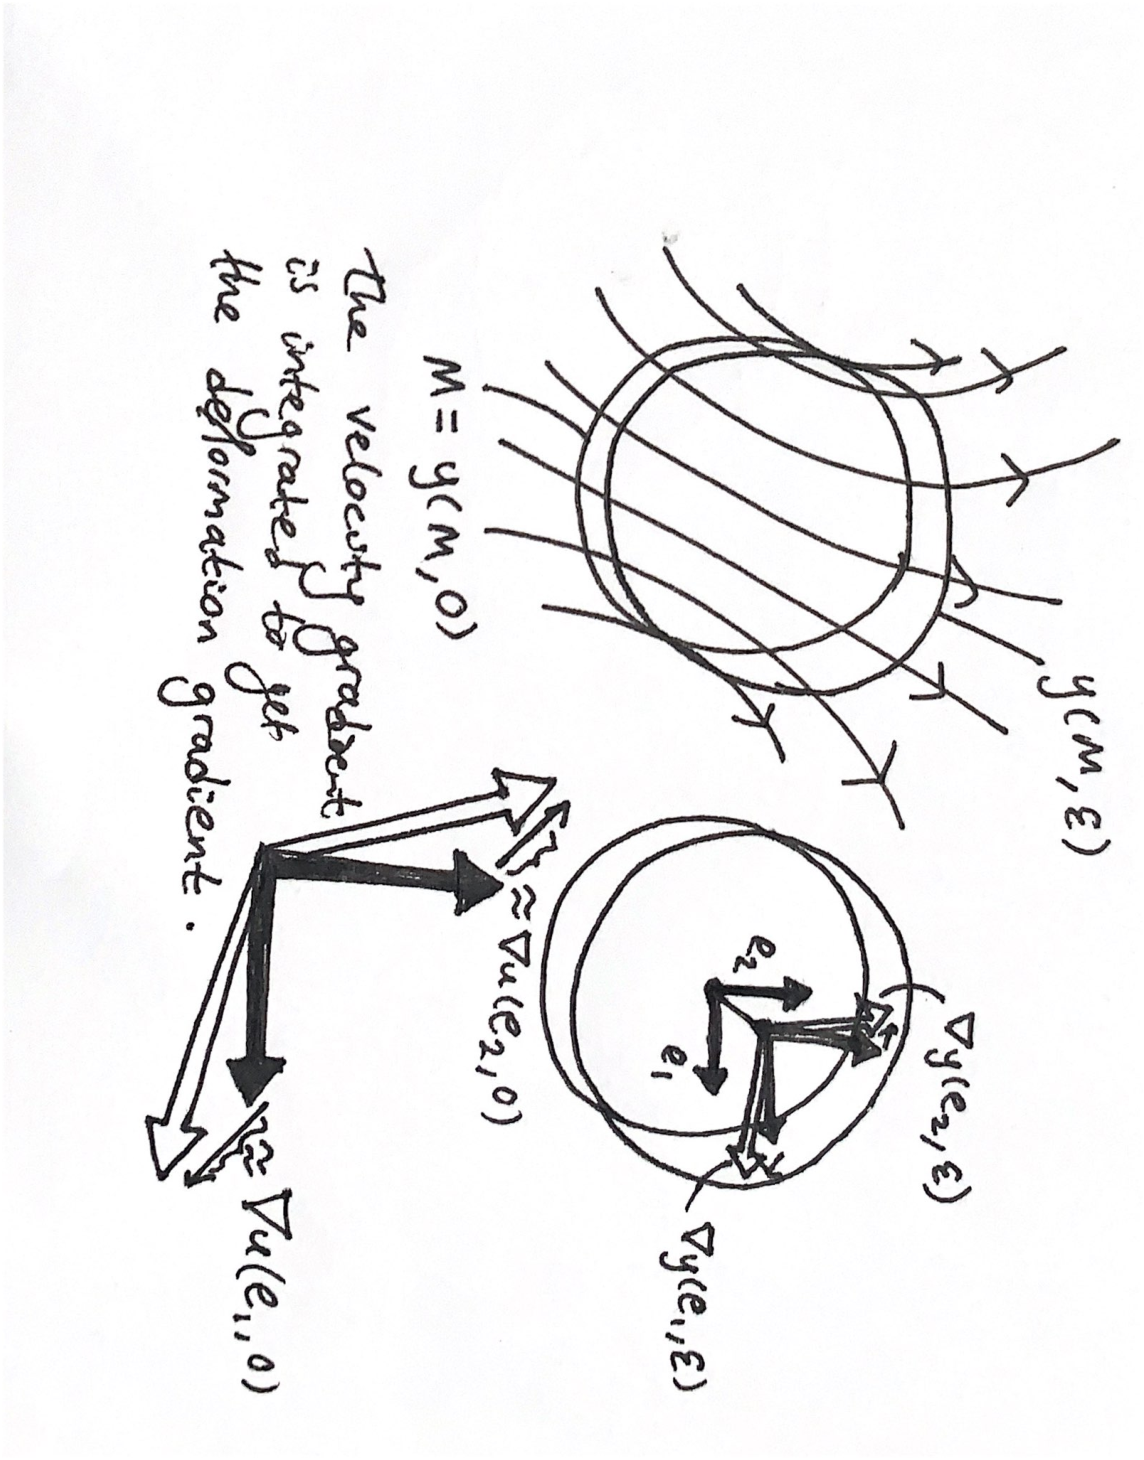
\includegraphics[angle=90,page=1,width=0.58\linewidth]{figures/1.pdf}
\end{center}

We can see that the term $\nabla u$ is a ``differential generator'' of the deformation gradient.
We call $\nabla u$, the spatial gradient of the Eulerian velocity, the \textit{velocity gradient}.

% Polar decomposition, symmetric and antisymmetric parts.
\subsection{Material points and material derivatives}\label{material_points}
\subsubsection{The material derivative}

Assuming an non-compressing flux function $u$ which transports quantity $\phi$, the differential form of the Reynolds transport theorem
\eqref{lagrangian_transport_differential} becomes
\begin{equation}
    \Part{\phi}{t} + \nabla\cdot(\phi u) = \Part{\phi}{t} + u\cdot\nabla\phi + \cancel{\phi \nabla\cdot u}.
\end{equation}
We define the \textit{material derivative} to be
\begin{equation}\label{material_derivative}
    \frac{D}{Dt} \coloneqq \Part{}{t} + u\cdot\nabla.
\end{equation}
It is a convention to leave the vector field $u$ implicit, as material derivatives are usually taken with respect to the velocity field.
This derivative \eqref{material_derivative} will turn out to measure ``per-volume'' quantities.

\subsubsection{Pieces of the continuum}
A \textit{material element} is a small piece of a continuum model which evolves with the displacement and flow.
In fluid dynamics this is also called a fluid parcel, although it should not be thought of as an object placed in the fluid, but
rather some tracer such as a non-diffusing dye.

% \vskip 0.2in
% (draw this)
% \vskip 0.2in
\begin{center}
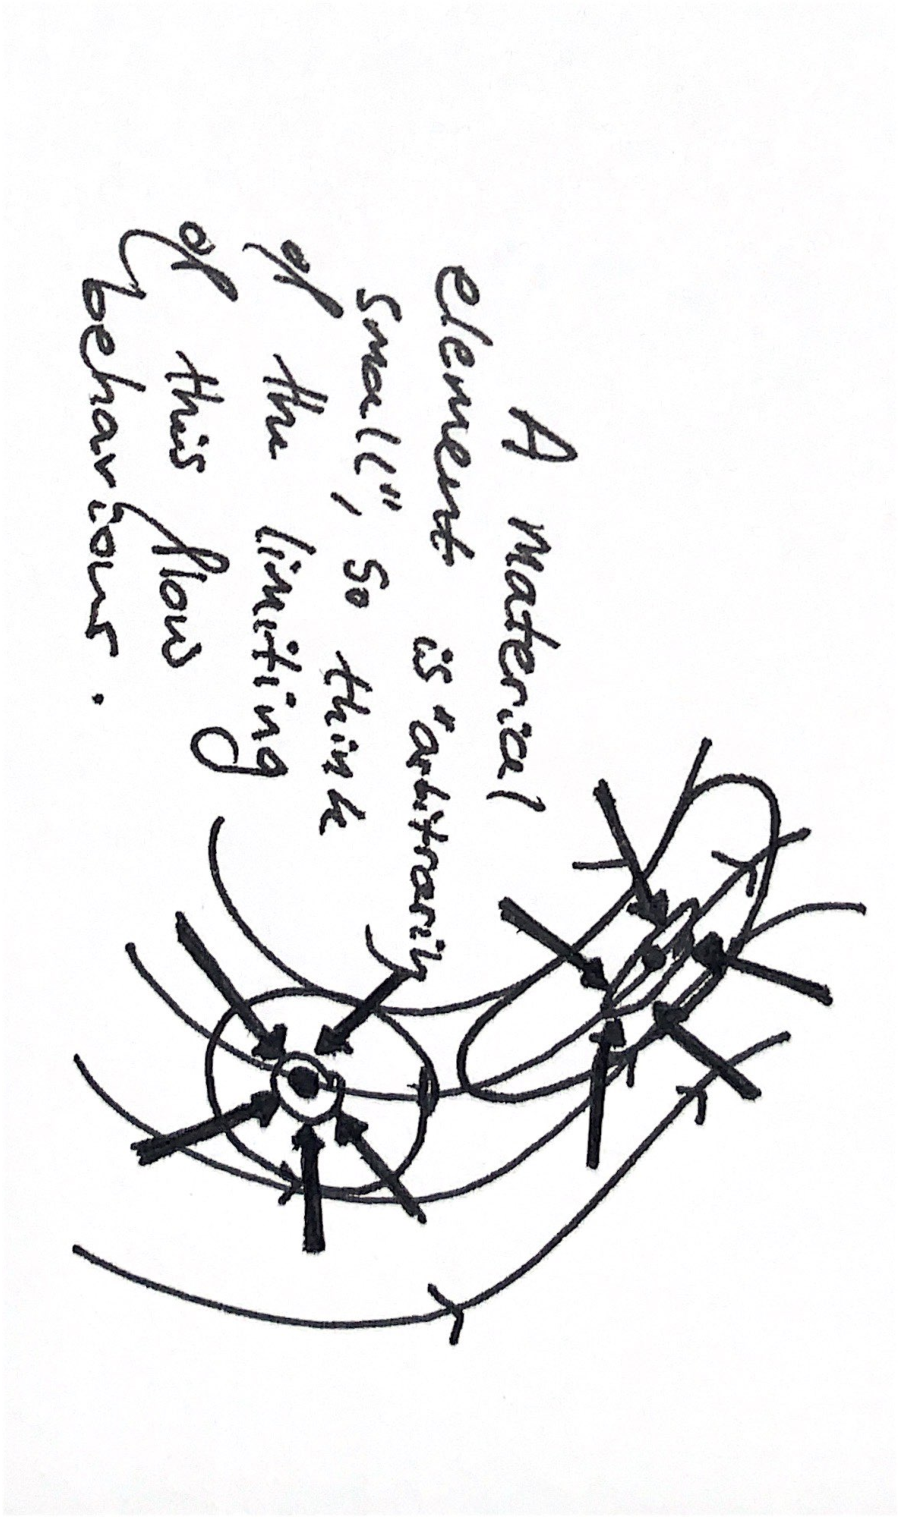
\includegraphics[angle=90,page=1,width=0.55\linewidth]{figures/2.pdf}
\end{center}

In continuum mechanics a \textit{material point} is the ideal point of the continuum, corresponding to some macroscopic averaging in physical models.
At a certain point, we can imagine an arbitrarily small fluid parcel being transported by the flow.
No matter how small this is, the parcel will still start to shear, expand, and contract due
to the flow.
The material derivative was defined as $\frac{D}{Dt} \coloneqq \Part{}{t} + u\cdot\nabla$. Notably this derivative contains no divergence term, and so does not
measure the
change of a quantity due to expansion and contraction of the arbitrarily small fluid parcel. Therefore we can think of the material derivative as acting
on \textit{per-volume} quantities.

% \vskip 0.2in
% (figure of a point mass flowing along a scalar field, and a mass with extent being compressed)
% \vskip 0.2in
\begin{center}
\includegraphics[page=2,width=0.66\linewidth]{figures/3.pdf}
\end{center}

\section{The dynamics of the continuum}

\subsection{Conservation of mass}
We will take for granted that there is some initial mass density function $\rho_0:M\rightarrow \mathbb{R}^+$
which we would like to conserve.
\subsubsection{The Lagrangian form of mass conservation}
As the position map $y$ evolves, for example under the action of Eulerian velocity field $u$ in the ODE \eqref{position_map_ode},
we would like a mass density function $\rho : N \rightarrow \mathbb{R}^+$ to be greater if the position map ``compresses'' the material,
and smaller if it ``stretches'' the material. Our aim is that the total mass measured in a control volume of $N$ is the same as in its initial configuration.
We can express this by the integral equation
\begin{equation}\label{lagrangian_mass_conservation}
    \int_{\omn} \rho_0(x)\,dx = \int_{y(\omn, t)} \rho(y, t)\,dy,
\end{equation}
where $y(\omn, t)$ denotes the domain pushed forward by the position map. By the usual change of variables formula we have
\begin{equation}\label{lagrangian_mass_conservation_cov}
    \int_{\omn} \rho_0(x)\,dx = \int_{\omn} \det(\nabla y)\rho(y(x,t), t)\,dx,
\end{equation}
where $J = \det(\nabla y)$ is the Jacobian, measuring the local change in the volume element due to the change of variables.

\vskip 0.2in
(draw this)
\vskip 0.2in

As \eqref{lagrangian_mass_conservation_cov} must hold identically for all $\Omega_0$, we have the localised conservation law
\begin{equation}\label{lagrangian_mass_conservation_local}
    \rho_0 = \det(\nabla y)\rho.
\end{equation}

\subsubsection{The Eulerian form of mass conservation}
Conservation law \eqref{lagrangian_mass_conservation_local} is simple. However, it is given in terms of absolute deformation gradient $\nabla y$.
Instead of asking how mass is distributed
in comparison to its initial configuration, we can ask how mass is transported by $u$.
This gives an instance of the continuity equation \eqref{continuity_equation}, where we have no source:
\begin{equation}\label{eulerian_mass_conservation}
    \frac{d}{dt} \int_{\omn} \rho \,dx + \int_{\pomn} \rho u\cdot \hat{n}\,dx = 0.
\end{equation}
With application of Stokes' theorem we have
\begin{equation}\label{eulerian_mass_conservation_local}
    \Part{\rho}{t} + \nabla \cdot (\rho u) = 0.
\end{equation}
Following \cite{leal}, there is a more geometrical statement of this equation, which will be useful when
we discuss ``material points''
By a divergence product rule \eqref{eulerian_mass_conservation_local} is equivalent to
\begin{equation}\label{eulerian_mass_conservation_local_material}
    \Part{\rho}{t} + u\cdot\nabla\rho + \rho\nabla\cdot u = 0
    \quad\Rightarrow\quad \frac{D\rho}{Dt} = -\rho\nabla\cdot u,
\end{equation}
where $\frac{D}{Dt}$ is the material derivative as defined in \eqref{material_derivative}.

\subsection{Conservation of linear momentum}

If we conserve the linear momentum $\rho u$, a ``quantity of motion'', under the flow of $u$, then we get a continuity equation
\begin{equation}\label{cauchy_continuity_traction}
    \eval{\frac{d}{dt}\left[\int_{\Omega_0(t)}\rho u\,dx\right]}_{t=0} = \int_{\omn(0)} \rho g\,dx + \int_{\pomn(0)}\hat{t}\,dx,
\end{equation}
a specific realisation of the Lagrangian continuity equation \eqref{lagrangian_transport}. The Lagrangian perspective is convenient
as it allows us to factor out certain forces on a moving piece of material. The term $g$ is a regular body force per unit mass, where $\rho g$ corresponds to
the source term $s$ in \eqref{lagrangian_transport}. The boundary term involving $\hat{t}$, however, has no analogue in the scalar continuity equation
\eqref{lagrangian_transport}.
This vector term $\hat{t}$ is called the \textit{traction} in continuum mechanics, and measures a local force exerted across the boundary
of the control volume due to the immediately adjacent material.

\subsubsection{The Euler-Cauchy stress principle}\label{stress_principle}
Clearly, in accord with Newton, we would like that two $\Omega_0$ and $\Omega_0^\prime$
which share a boundary element should have equal and opposite tractions across that boundary element.
Since the normal $\hat{n}$ represents a boundary element, and is negative for the opposite element, if $\hat{t}$ is linear in $\hat{n}$ we have this required
property. We can then let \eqref{cauchy_continuity_traction} become
\begin{equation}\label{cauchy_continuity}
    \eval{\frac{d}{dt}\left[\int_{\Omega_0(t)}\rho u\,dx\right]}_{t=0} = \int_{\omn(0)} \rho g\,dx + \int_{\pomn(0)}\sigma:\hat{n}\,dx
\end{equation}
where $\sigma$ is termed the \textit{Cauchy stress tensor}.


% <<<
\subsubsection{Differentializing the Cauchy momentum equation}
By application of the Reynolds transport theorem \eqref{reynolds_transport_theorem_tensor} to \eqref{cauchy_continuity} we get
\begin{equation}\label{cauchy_continuity_eulerian}
    \int_{\Omega_0(0)}\Part{(\rho u)}{t}\,dx + \int_{\partial\Omega_0(0)}\rho u (u\cdot \hat{n})\,dx = \int_{\Omega_0(0)} \rho g\,dx + \int_{\pomn(0)} \sigma:\hat{n}\,dx.
\end{equation}
Differentializing \eqref{cauchy_continuity_eulerian}, by our previously derived tensor identities, gives
\begin{equation}\label{cauchy_continuity_differential}
    \Part{(\rho u)}{t} + \nabla \cdot (\rho u\otimes u) = \rho g + \nabla\cdot\sigma.
\end{equation}
This is called the \textit{conservative form} of the Cauchy momentum equation.
We can derive another, possibly more convenient form of \eqref{cauchy_continuity_differential} using the fact that
$\rho$ is conserved and has no source. Here, this will be derived purely algebraically, although the final form of the equation
has a useful interpretation. Expanding the partial derivative
$$
    \Part{(\rho u)}{t} = \rho\Part{u}{t} + u\Part{\rho}{t}
$$
is simple. The tensor divergence $\nabla \cdot (\rho u\otimes u)$ is defined such that
$$
    \int_{\Omega_0} \nabla \cdot (\rho u\otimes u)\,dx = \int_{\pomn} (\rho u\otimes u) : \hat{n}\,dx = \int_{\pomn} \rho u (u\cdot\hat{n})\,dx
$$
for arbitrary control volumes $\Omega_0$. As $\Omega_0$ becomes small, we can separately assume $u$ and $\rho u$ are constant
to derive
$$
    \int_{\pomn} \rho u (u\cdot\hat{n})\,dx = u\int_{\pomn}(\rho u)\cdot\hat{n}\,dx
                                              + \rho u\cdot \int_{\pomn} u\hat{n}\,dx \quad+\quad\cdots
$$
where a trailing term becomes neglible for a small control volume. This gives a ``tensor product rule'' for the divergence,
\begin{equation}\label{cauchy_divergence_tensor_product}
    \nabla\cdot (\rho u \otimes u) = u\nabla\cdot (\rho u) + \rho u\cdot\nabla u.
\end{equation}
Equation \eqref{cauchy_continuity_differential} then becomes
$$
    \rho\Part{u}{t} + u\Part{\rho}{t} + u\nabla\cdot (\rho u) + \rho u\cdot\nabla u = \rho g + \nabla\cdot\sigma.
$$
Noting that $\Part{\rho}{t}$ is already given by continuity equation \eqref{eulerian_mass_conservation_local}
$$\Part{\rho}{t} = -\nabla\cdot(\rho u),$$
as mass is transported by $u$ and has no source, we get
$$
    \rho\Part{u}{t} -\cancel{u\nabla(\rho u)} + \cancel{u\nabla\cdot (\rho u)} + \rho u\cdot\nabla u = \rho g + \nabla\cdot\sigma.
$$
Finally, the material derivative as defined in section (ref) is helpful in simplifying the above to
\begin{equation}\label{cauchy_continuity_differential_material}
    \rho\frac{Du}{Dt} = \rho g + \nabla\cdot\sigma.
\end{equation}
This form of \eqref{cauchy_continuity_differential} is called the \textit{convective form} of the Cauchy momentum equation, and is more obviously a form of $F = ma$.
% From this derivation we have the identity
% \begin{equation}\label{mass_conserved_linear_momentum_identity}
%     \Part{(\rho u)}{t} + \nabla\cdot(\rho u\otimes u)
%     = \rho\frac{Du}{Dt}
% \end{equation}
% when mass density $\rho$ is conserved by $u$. The left-hand-side in \eqref{mass_conserved_linear_momentum_identity} is the differentialized Reynolds transport \eqref{reynolds_transport_theorem_tensor_differential},
% which measures the change in total linear momentum when following a small control volume that begins at a point $x^*$ and flows with $u$.
% If we integrate both sides over a control volume and apply the Reynolds transport theorem, we get
% \begin{equation}\label{mass_conserved_linear_momentum_identity_integral}
%     \eval{\frac{d}{dt}\left[\int_{\omn(t)} \rho u\,dx\right]}_{t=0} = \int_{\omn(0)} \rho \frac{Du}{Dt}\,dx.
% \end{equation}
% >>>
Recall that the material derivative is defined as
    $$\frac{D}{Dt} \coloneqq \Part{}{t} + u\cdot \nabla,$$
which measures the rate of change of a pointwise quantity from the perspective of a particle moving with the flow field $u$.
The equation \eqref{cauchy_continuity_differential_material} then says that, if the continuum consists of idealised points
each with a certain linear momentum (in the particle sense), deflection of their inertial path is due only to the application
of a body force $\rho g$ at this point, and a total traction force exerted by the surrounding material.

\subsection{Constitutive relations}\label{constitutive_relations}
The conservation equations derived are conservation of mass \eqref{eulerian_mass_conservation_local} and conservation of linear momentum \eqref{cauchy_continuity_differential_material}.
Here the equations are given in their typical differential form for flow problems, with the Eulerian perspective of mass conservation, and the
convective form of linear momentum conservation:
\begin{equation}\label{conservation_system}
\begin{split}
    \frac{D\rho}{Dt} + \rho\nabla\cdot u = 0 &\quad\text{(Conservation of mass)},
    \\
    \rho\frac{Du}{Dt} = \rho g + \nabla\cdot\sigma &\quad\text{(Conservation of linear momentum)}.
\end{split}
\end{equation}
The unknowns include mass density $\rho$ and velocity $u$, described by $1 + d$ scalar functions where $d$ is the dimension of the domain.
We can see there are $1 + d$ equations by expanding $u$ in terms of components in some basis.
\begin{align*}
\begin{split}
    \rho\frac{Du_i}{Dt} = \rho g_i + \left(\nabla\cdot\sigma\right)_i &\quad\text{(Conservation of linear momentum components)},
    \\
    i=1,\cdots,d. &
\end{split}
\end{align*}
When $g$ and $\sigma$ are known, this system is well-formed, but not very interesting.
This effectively models a continuum of non-interacting material points, with a linear-momentum-introducing source function $\rho g + \nabla\cdot \sigma$.
However, we usually let $g$ be known (as this is a per-mass external body force, for example gravity), and the Cauchy stress tensor $\sigma$ be unknown.
This gives $d^2$ more unknowns, so the system is heavily underdetermined. In effect, the system \eqref{conservation_system} is
underdetermined because we don't have a specific material in mind.

\subsubsection{Constitutive relations}
A specification of the Cauchy stress tensor $\sigma$ is called a \textit{constitutive relation},
as $\sigma$ depends on the ``material constitution''.
A constitutive relation specifies how the material configuration
induces forces on the material, or rather, how kinematics is related to dynamics. With $\sigma$ specified, the Cauchy momentum equation \eqref{cauchy_continuity_differential_material} becomes well-posed
(however, in general, $\sigma$ may depend on new variables such as temperature, requiring further equations).

% \subsubsection{Deviatoric and volumetric stresses}
% Suppose that the tractions are determined only by the velocity gradient,
%     $$\sigma = \sigma(\nabla u).$$
% We have the symmetric-antisymmetric splitting of the velocity gradient
% \newcommand{\usym}{\frac{1}{2}\left(\nabla u + \nabla u^T\right)}
% \newcommand{\uantisym}{\frac{1}{2}\left(\nabla u - \nabla u^T\right)}
% \begin{align*}
%     \nabla u = \usym + \uantisym.
% \end{align*}
% The symmetric term $\usym$ can be thought of as differential generator of stretching (as the exponential of a symmetric matrix is symmetric-positive-definite),
% and the antisymmetric term $\uantisym$ can be thought of as a differential generator of rotations (as the exponential of an antisymmetric matrix is orthogonal).

% \subsubsection{Pressure in incompressible materials}
% TODO: Shorten or remove
% 
% 
% The concept of pressure will be very important in our discussion of the Navier-Stokes equations, so we introduce it
% here. A detailed derivation of the pressure is given in terms of Stokes flow in section \ref{pressure_derivation}.
% 
% If we require the velocity field $u$ of the position map $x$ to be non-compressing (as described in section (ref)),
% then we add to our model equations the constraint
% \begin{equation}\label{noncompressing_velocity}
%     \nabla \cdot u = 0.
% \end{equation}
% We proceed by analogy to a simple mechanical system.
% The state of a pendulum of mass $m$ might be described by two spatial variables $X$ and $Y$ with a constraint
%     $$X^2 + Y^2 = 1.$$
% Given a differentiable pendulum motion, the linear momenta $mv_X$ and $mv_Y$ clearly cannot be constant, as then the pendulum
% would ``fly out'' of its arc.
% From the perspective of the $X,Y$ coordinate system there exists ``virtual forces'' which are exactly those that are needed
% to maintain constraints. These forces have no necessary physical interpretation, as the pendulum model does not explicitly reference
% the tension of the pendulum rod, but are rather those strong forces that must ``come from somewhere'' such that the constraints
% are satisfied.
% 
% \vskip 0.2in
% (figure)
% \vskip 0.2in
% 
% From a constraint on position $(X,Y)$ we can derive a constraint on velocity $(v_X,v_Y)$ by noting that the velocity must stay inside
% the tangent plane in the configuration space. In this case, we require
% \begin{equation}\label{pendulum_velocity_constraint}
%     Xv_X + Yv_Y = 0.
% \end{equation}
% (--- add Lagrange multipliers to the system, then pressure here is a sort of Lagrange multiplier).
% The continuum velocity constraint \eqref{noncompressing_velocity} is completely analogous to \eqref{pendulum_velocity_constraint}.
% Motions of $x$ are restricted to those which do not compress mass. Clearly, our (per-point) linear momentum $\rho u$
% cannot be constant except in simple parallel flows, implying the existence of some virtual (per-point) force.
% We call this force the \textit{pressure} $p$, and we are now solving for $\rho$, $u$, and $p$ in a coupled system of equations
% \eqref{cauchy_continuity_differential_material} and \eqref{noncompressing_velocity}, repeated here:
% \begin{align*}
%     \rho\frac{Du}{Dt} = \rho g + \nabla\cdot\sigma,\quad
%         \nabla \cdot u = 0.
% \end{align*}
% As there is no explicit mention of $p$, it must be part of the constitutive relation for $\sigma$.
% We let $\sigma$ be
% \begin{align*}
%     \sigma = -pI + \tau \quad\Rightarrow\quad \nabla\cdot\sigma = -\nabla p + \nabla\cdot \tau,
% \end{align*}
% where $I$ is the identity tensor and $\tau$ is called the \textit{deviatoric} component of the Cauchy stress tensor.
% $\tau$ is chosen such that the pressure $p$ entirely encapsulates the isotropic forces which push material volumes apart.

\subsubsection{Completing the equations}
We have so far been working quite generally with the forms of continuum mechanics models and their constraints. Although we have made some assumptions
(for example, we require $\sigma$ to be a purely local function, an idealisation due to Cauchy [ref]), we must so far leave
our systems underdetermined.
In the next chapter, we will
investigate an important constitutive relation for the stress $\sigma$, forming what is called a \textit{Navier-Stokes fluid},
giving a complete system of equations called the \textit{Navier-Stokes equations}.

\chapter{The Navier-Stokes equations}

% \section{The kinematics of flow}
% \subsection{Vorticity}
% \subsection{The Helmholtz decomposition}
% \subsubsection{The stream function}
% \subsubsection{The velocity potential}

\section{Introduction}
The incompressible Navier-Stokes equations model the motion of a common kind of viscous fluid called a \textit{Newtonian fluid}.
They are:
\begin{itemize}
\item The Cauchy momentum equation \eqref{cauchy_continuity_differential_material} for constant mass density $\rho$ and velocity $u$,
\item an incompressibility constraint $\nabla\cdot u = 0$ and unknown pressure $p$,
\item and a concrete constitutive relation for the deviatoric stress $\tau$.
\end{itemize}
In anticipation, their common form is
\begin{equation}\label{navier_stokes}
    \rho\frac{Du}{Dt} = - \nabla p + \nabla\cdot\tau + \rho g,\quad \nabla\cdot u = 0,
\end{equation}
where $\tau$ is defined by Stokes' constitutive relation
\begin{equation}\label{stokes_constitutive_relation}
    \tau = \mu\left(\nabla u + \nabla u^T\right),
\end{equation}
where $\mu$ is called the \textit{viscosity}, and $\nabla u$ is the velocity gradient defined in section \ref{deformation_and_velocity_gradients},
measuring the local deformation of a small control volume under
the flow of $u$. We will assume their domain is a subset of $\mathbb{R}^d$, where typically $d = 2$ or $3$, although the Navier-Stokes equations can be solved
in curved domains (see \cite{stam}).
Alongside a domain and appropriate initial and boundary conditions, the Navier-Stokes equations \eqref{navier_stokes}
form a concrete flow problem which
can be solved numerically, or in special situations analytically.

\section{Constitutive relations for the Navier-Stokes equations}
We begin with the standard conservation equations of mass and linear momentum, \eqref{conservation_system}:
\begin{equation*}
\begin{split}
    \frac{D\rho}{Dt} + \rho\nabla\cdot u = 0 &\quad\text{(Conservation of mass)},
    \\
    \rho\frac{Du}{Dt} = \rho g + \nabla\cdot\sigma &\quad\text{(Conservation of linear momentum)}.
\end{split}
\end{equation*}
As discussed in section \ref{constitutive_relations}, we need to specify $\sigma$ such that the system is well-formed. Firstly, we replace the
conservation of mass equation with the incompressibility constraint
\begin{equation*}
    \nabla \cdot u = 0.
\end{equation*}
Assuming a constant mass density $\rho$, this also expresses mass conservation. This will preclude phenomena such as acoustic waves in the fluid,
but is a good approximation for many studies of fluid motion (see Batchelor \cite{batchelor}).

\subsection{Conservation of angular momentum}
Angular momentum is traditionally presented in terms of rigid bodies, bodies subject to a distance-preserving constraint between
material points. It is the moment of linear momentum.

The discussion in section \ref{material_points} indicates that we can think of a very small rigid body at a material point, subject to the flow.
This will be subject to a ``spin force''.

Let the material point be $c \in \mathbb{R}^d$, which will act as a ``centre of mass', and let $c \in \Omega_0$.
Define $\bar{x} \coloneqq x - c$.
Define the moment of linear momentum as
\begin{equation}\label{moment_of_linear_momentum}
    \int_{\omn} \bar{x} \wedge \left(\rho u\right)\,dx.
\end{equation}
The symbol $\wedge$ indicates the cross product, whose value should be thought of as a pseudo-vector or ``plane with magnitude''.
We will call this the angular momentum of the control volume $\omn$.
We repeat here an integral form of linear momentum conservation, which already must hold:
\begin{equation}\label{linear_momentum_for_angular}
    \int_{\omn(0)} \Part{(\rho u)}{t}\,dx + \int_{\pomn(0)} \rho u (u\cdot \hat{n})\,dx
    = \int_{\omn(0)} \rho g\,dx + \int_{\pomn(0)} \sigma \hat{n}\,dx.
\end{equation}
It is simple to derive an angular momentum conservation equation, just by taking moments of each vector quantity:
\begin{equation}\label{moment_of_linear_momentum_sources}
    \int_{\omn(0)} \bar{x} \wedge \Part{(\rho u)}{t}\,dx + \int_{\pomn(0)} \bar{x} \wedge \left(\rho u\right)\left(u\cdot \hat{n}\right)\,dx
    = \int_{\omn(0)} \bar{x} \wedge \left(\rho g\right)\,dx + \int_{\pomn(0)} \bar{x} \wedge \left(\sigma \hat{n}\right)\,dx.
\end{equation}
(This precludes the introduction of surface and body couples which induce no linear momentum but do induce angular momentum
\cite{leal}. We ignore these torques.)
\\
If \eqref{linear_momentum_for_angular} holds, should \eqref{moment_of_linear_momentum_sources} hold automatically?

(... figure)
\begin{center}
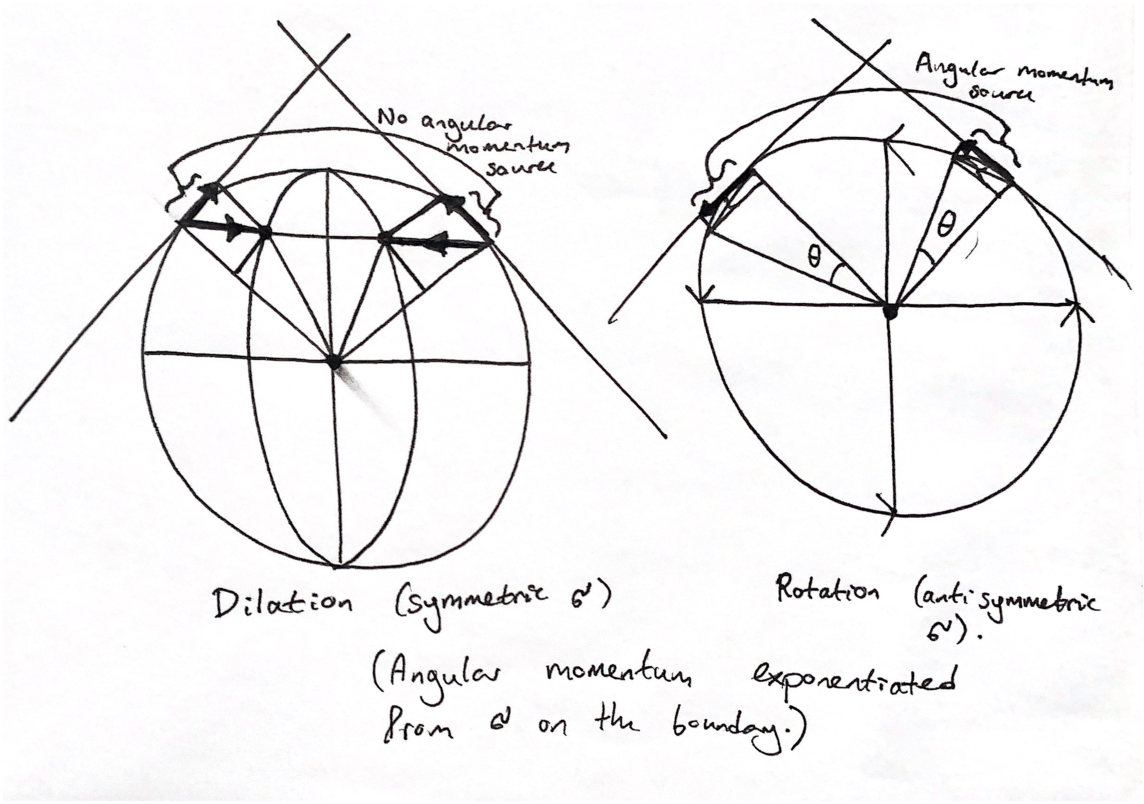
\includegraphics[page=1,width=0.7\linewidth]{figures/3.pdf}
\end{center}


% If the control volume follows the flow, the Reynolds transport theorem \eqref{reynolds_transport_theorem} gives a rate of change of angular momentum:
% \begin{equation}\label{moment_of_linear_momentum_reynolds}
%     \frac{d}{dt}\eval{\left[\int_{\omn(t)} \bar{x} \wedge \left(\rho u\right)\,dx\right]}_{t=0}
%     % = \int_{\omn(0)} \left(x - c\right)\wedge \left(\rho g\right)\,dx + \int_{\pomn(0)} \left(x - c\right) \wedge \hat
%     = \int_{\omn(0)} \bar{x} \wedge \Part{(\rho u)}{t}\,dx + \int_{\pomn(0)} \bar{x} \wedge \rho u (u\cdot \hat{n})\,dx.
% \end{equation}
% The source terms of linear momentum are body forces $\rho g$ on the interior and tractions $\hat{t}$ on the boundary.
% Therefore we have an explicit equation for the rate of change of angular momentum, which we equate to the right-hand-side of
% \eqref{moment_of_linear_momentum_reynolds}:
% \begin{equation}\label{moment_of_linear_momentum_sources}
%     \int_{\omn(0)} \bar{x} \wedge \Part{(\rho u)}{t}\,dx + \int_{\pomn(0)} \bar{x} \wedge \rho u (u\cdot \hat{n})\,dx
%     = \int_{\omn(0)} \bar{x} \wedge \left(\rho g\right)\,dx + \int_{\pomn(0)} \bar{x} \wedge \left(\sigma \hat{n}\right)\,dx.
% \end{equation}
% By the Euler-Cauchy stress principle (section \ref{stress_principle}), we have let the traction $\hat{t} = \sigma \hat{n}$.
% For comparison, we repeat here an integral form of linear momentum conservation, which already must hold:
% \begin{equation*}
%     \int_{\omn(0)} \Part{(\rho u)}{t}\,dx + \int_{\pomn(0)} \rho u (u\cdot \hat{n})\,dx
%     = \int_{\omn(0)} \left(\rho g\right)\,dx + \int_{\pomn(0)} \sigma \hat{n}\,dx.
% \end{equation*}


\section{Scaling and dimension}
\subsection{The Reynolds number}

\section{Stokes flow and the meaning of pressure}\label{pressure_derivation}
If we assume that the advective term $u\cdot \nabla u$ in the incompressible Navier-Stokes equations is ``small'',
we can ignore it and derive the linear \textit{unsteady Stokes equations}:
\begin{equation}\label{unsteady_stokes}
    \rho\Part{u}{t} = \mu\Delta u + \rho g - \nabla p, \quad \nabla\cdot u = 0.
\end{equation}
We are assuming validity for low Reynolds number $Re \ll 1$, where convective behaviour is neglible compared to the viscous forces, which for a
Navier-Stokes fluid ``diffuse'' the linear momentum. Setting the left-hand-side of \eqref{unsteady_stokes} to zero results in the \textit{steady Stokes equations}
\begin{equation}\label{steady_stokes}
    \mu\Delta u + \rho g - \nabla p = 0,\quad \nabla\cdot u = 0.
\end{equation}
Time-dependent equation \eqref{unsteady_stokes} can be thought of as a ``gradient descent'' to find the steady Stokes flow \eqref{steady_stokes}.
The steady Stokes equation is a constrained vector Poisson equation, where we have introduced pressure $p$ explicitly.
It is well-known, by Dirichlet's principle, that we can think
of a weak solution to the unconstrained vector Poisson equation as a minimiser of the Dirichlet energy,
\begin{equation}
\begin{aligned}
& \underset{u}{\text{minimize}}
& & E(u) =  \frac{\mu}{2} \inner{\nabla u, \nabla u} - \inner{u, \rho g}.\\
\end{aligned}
\end{equation}
\newcommand{\energygradient}{\frac{\delta E}{\delta u}}
We can validate this by computing the Euler-Lagrange equations:
\begin{align*}
    % \frac{\delta E}{\delta u} = \Part{\fancyL}{u} - \frac{d}{dx}\Part{\fancyL}{\nabla u}
    % notation?
    \frac{\delta E}{\delta u} = \Part{\fancyL}{u} - \frac{d}{dx}\Part{\fancyL}{u_x}
                              = -\rho g - \mu\Delta u = 0.
\end{align*}
We now introduce the incompressibility constraint $\nabla \cdot u = 0$, giving the constrained minimization
\begin{equation}\label{stokes_flow_optimization}
\begin{aligned}
& \underset{u}{\text{minimize}}
& & E(u) =  \frac{\mu}{2} \inner{\nabla u, \nabla u} - \inner{u, \rho g}\\
& \text{subject to}
& & \nabla\cdot u = 0.
\end{aligned}
\end{equation}
It is not immediately obvious how to form the constrained Euler-Lagrange equations here, as $\nabla\cdot$ is a differential operator.
We cannot just write
    $$\text{``}\frac{\delta E}{\delta u} = \lambda\nabla\cdot\text{''}$$
for scalar function $\lambda$, as we can with a pointwise linear constraint such as $u\cdot v = 0$ for some vector field $v$. However, this is just a problem of
notation. The evaluation of energy change with perturbations is defined as
\begin{align*}
    \inner{\frac{\delta E}{\delta u}, \delta u} = \int_\Omega \frac{\delta E}{\delta u}\cdot\delta u\,dx.
\end{align*}
We want this measure of energy change to be purely a divergence measure, up to a scalar multiplier $\lambda$:
\begin{equation}\label{el_pressure_constrained_div}
    \int_\Omega \frac{\delta E}{\delta u}\cdot\delta u\,dx = \int_\om \lambda \nabla\cdot \delta u\,dx.
\end{equation}
This means
that virtual displacements with $\nabla\cdot\delta u = 0$ will not cause an energy change, which is the condition that
we want for a stationary point.
We can now apply integration by parts to \eqref{el_pressure_constrained_div}, assuming that $\delta u$ vanishes on the boundary of the domain, to get
\begin{equation}
    \int_\Omega \frac{\delta E}{\delta u}\cdot\delta u\,dx = -\int_\om \nabla\lambda \cdot \delta u\,dx.
\end{equation}
We can now reasonably apply the localisation step to get the constrained Euler-Lagrange equations
\begin{equation}
\begin{split}
           \frac{\delta E}{\delta u} = -\nabla \lambda
    \quad\equiv\quad \mu\Delta u + \rho g - \nabla \lambda = 0.
\end{split}
\end{equation}
Along with the constraint $\nabla\cdot u = 0$, this is just the steady Stokes equations \eqref{steady_stokes}, where $\lambda = p$! We can see that the pressure $p$
is actually
a Lagrange multiplier, which measures a virtual force that responds to virtual displacements which would break the constraint of incompressibility.
In fact, we may think of this as a derivation of the pressure.

\subsubsection{Alternative direct derivation in terms of a modified energy}
Previously, we emphasized the meaning of the Lagrange multiplier. One utility of Lagrange's methods is their automated calculational power.
It is standard to express that a solution to the optimization
problem \eqref{stokes_flow_optimization}, with a differentiable equality constraint, is a stationary point of the modified energy
\begin{equation}\label{stokes_flow_modified_energy}
    L(u, \lambda) \coloneqq \frac{\mu}{2} \inner{\nabla u, \nabla u} - \inner{u, \rho g} - \inner{\lambda, \nabla\cdot u}.\\
\end{equation}
We can take an evaluated first variation with respect to $u$ to get
\begin{align*}
    \inner{\frac{\delta L}{\delta u}, \delta u} = \inner{-\rho g - \mu\Delta u, \delta u} - \inner{\lambda, \nabla\cdot\delta u},
\end{align*}
which by integration by parts becomes
\begin{equation}
    \inner{\frac{\delta L}{\delta u}, \delta u} = \inner{-\rho g - \mu\Delta u + \nabla \lambda, \delta u}.
\end{equation}
We then get
\begin{equation}
\begin{split}
    \frac{\delta L}{\delta u} &= -\rho g - \mu\Delta u + \nabla \lambda = 0,\\
    \frac{\delta L}{\delta \lambda} &= -\nabla\cdot u = 0,
\end{split}
\end{equation}
which are the steady Stokes equations \eqref{steady_stokes} with pressure $p = \lambda$.



\subsection{Application to hydrostatics}
For example, we may imagine the steady Stokes equations modelling a calm sea with a flat seabed.
We can let the body force be gravity described by a potential $\phi$:
    $$\rho g = -\nabla \phi.$$
If we make a perturbed displacement of the velocity field at the bottom of the ocean, supposing that some volume of water
is beginning to expand,
we are working against gravity as well as our virtual force, pressure.

\vskip 0.2in
(draw this)
\vskip 0.2in



% Navier-Stokes in expanded differential form for Cartesian coordinates. Maybe useful for finite differences.
% Working backwards to the weak form doesn't make much sense.
% \subsection{Kinds of fluids}
% \subsubsection{Incompressible fluids}
% \subsubsection{Inviscid flow}
% \subsubsection{Irrotational flow}
% \subsubsection{Steady flow}
% \subsubsection{Viscous flow and Newtonian fluids}

\chapter{The finite element method}
\section{Introduction}

Consider a single conservation law as described in section \ref{conservation_laws}. This law
was given in two forms, ``integral'' \eqref{continuity_equation}:
\begin{equation*}
    \frac{d}{dt} \int_{\Omega_0} \phi\,dx = \int_{\Omega_0} s\,dx + \int_{\pomn} \phi j \cdot \left(-\hat{n}\right)\,dx,
\end{equation*}
and ``differential'' \eqref{continuity_equation_differential}:
\begin{equation*}
    \Part{\phi}{t} = s - \nabla\cdot (\phi j).
\end{equation*}
Thinking about \eqref{continuity_equation} will lead to Galerkin methods, which include finite volumes, finite elements, and spectral methods.
Thinking about \eqref{continuity_equation_differential} will lead, primarily, to the finite difference method, historically the first and
still very important in applications. We will discuss the latter first.

\subsection{Discretization of the differential form}
The finite difference method will take equation \eqref{continuity_equation_differential} and, for example, expand the divergence by Gauss' theorem
\eqref{gauss_euclidean_divergence}:
$$
    \nabla \cdot j = \Part{j_x}{x} + \Part{j_y}{y} + \Part{j_z}{z}.
$$
The approximate solution may be represented by a number of samples on the domain, for example, a grid. The term
$j_x$ above could then be approximated by a secant, for example a central difference.

\vskip 0.2in
(draw this)
\vskip 0.2in

However, we have not necessarily given a real interpretation of what the solution samples at grid points say about the solution everywhere.
They could be a coefficients of, for example, hat basis functions.

\vskip 0.2in
(draw this)
\vskip 0.2in

Yet a finite difference discretization of \eqref{continuity_equation_differential} may not take this into account at all. One might feel that
limits have been taken too soon, and that the integral form \eqref{continuity_equation} gives clearer routes to discretizations which
have geometric meaning.

\subsection{Discretization of the integral form}
The integral conservation law \eqref{continuity_equation} is a geometric statement about fluxes
of quantity $\phi$ by $j$, quantified over arbitrary control volumes $\Omega_0$.
We have an infinite number of control volumes, and therefore equations which must hold, and an infinite-dimensional
space of solutions to choose from. A key idea, then, is to choose a finite number of equations and a finite-dimensional subspace of possible solutions.
A supposed solution will be represented by the coefficients of some choice of basis functions for the subspace. Each equation will be checked exactly against this supposed solution.

\vskip 0.2in
(figure)
\vskip 0.2in

Finite element methods, and more generally Galerkin methods, live comfortably in the language of weak solutions, integral forms of partial differential equations,
and the calculus of variations. Some methods of this kind will be derived in the subsequent sections, investigating discretizations of the integral forms
of some physical PDEs. In order:
\begin{itemize}
    \item The linear Poisson equation: Finite volumes, finite elements, linear systems.
    \item The linear Stokes equations: FEM with constraints, time-dependence.
    \item A non-linear Poisson equation: Non-linear FEM.
    \item A non-linear heat equation: Non-linear, time-dependent FEM.
    \item The Burgers equation: Introduces shocks and the numerical effect of viscosity.
\end{itemize}
This is in order to build up concepts to solve the non-linear time-dependent Navier-Stokes equations.

\section{Solving the Poisson equation}
% The weak form is exactly analogous to perturbation principle in the principle of least action.
% To actually be an instance of the principle of least action, we need a Lagrangian. For example, the Poisson
% equation is the Euler-Lagrange equation of the Dirichlet energy.
Poisson's equation is a steady-state version of the heat equation.
Through this investigation we will derive many of the tools and ideas underlying general Galerkin methods.
In particular we will derive a \textit{finite volume method} and a \textit{finite element method} from first principles.
In anticipation, some results are shown below:

\vskip 0.2in
(visualisations)
\vskip 0.2in

We will defer the important step of analysis of our methods' convergence and stability to a later section.

\subsection{Deriving the Poisson equation through diffusion processes}
A diffusion process ``levels out'' some quantity, such as temperature or some chemical concentration. We can intuitively think of a diffusion as a
progressive ``blurring''
such as in a camera defocus, and in fact many common image processing techniques use diffusion PDEs from physics \cite{tum}. We will stick with
the notion of temperature $h$ as the diffused quantity.
\textit{Fick's law of diffusion} is a constitutive relation giving the bulk flux of temperature $h$ as proportional to the negative gradient:
    $$hj = -\mu\nabla h,$$
where $\mu$ is called the diffusion coefficient.
This is one way of saying that the temperature tends to level out.
If we form a continuity equation \eqref{continuity_equation} for temperature, with source $s$, we get
\begin{equation}\label{heat_equation_integral}
    \frac{d}{dt} \int_{\Omega_0} h\,dx = \int_{\Omega_0} s\,dx + \int_{\pomn} \mu \nabla h \cdot \hat{n}\,dx,
\end{equation}
which by application of Stokes' theorem becomes
\begin{equation}\label{heat_equation_differential}
    \frac{dh}{dt} = s + \nabla \cdot \left(\mu \nabla h\right).
\end{equation}
If we further assume that the diffusion coefficient $\mu$ is constant, we get
\begin{equation}\label{heat_equation_differential_constant}
    \frac{dh}{dt} = s + \mu\nabla \cdot \nabla h = s + \mu\Delta h,
\end{equation}
which is the standard heat equation.
The steady-state heat equation is then
\begin{equation}\label{poisson_equation}
    -\Delta h = f,
\end{equation}
where we let $f = s/\mu$ in the above. Equation \eqref{poisson_equation} is called the Poisson equation,
which models steady-state diffusion processes and can be used to calculate gravitational or electrostatic potential fields.
In integral form, ``undoing'' the application of Stokes' theorem above, the Poisson equation is
\begin{equation}\label{poisson_equation_integral}
    \int_{\pomn} -\nabla h\cdot \hat{n}\,dx = \int_{\omn} f\,dx.
\end{equation}
Form \eqref{poisson_equation_integral} clearly shows that we are calculating a steady state,
as we are solving for $h$ such that the amount of heat that leaves $\Omega_0$ is the amount created by the source function.
This form will be the most convenient for our numerical methods.

\subsection{Discretizing the Poisson equation}\label{discretizing_poisson}
Equation \eqref{poisson_equation_integral} is quantified over arbitrary control volumes $\Omega_0$.
A simple idea is to break the domain $\Omega$ up into small cells $\Omega_1,\cdots,\Omega_n$, and check that the flux integral holds over each of these.
We will then have $n$ equations on $h$. As this system will be underdetermined ($h$ has infinite degrees of freedom), we must
restrict $h$ to what we will call a ``test space'',
    $$\Phi = \text{span}\left\{\phi_1,\cdots,\phi_n\right\}.$$
The basis functions $\phi_i$ should generate a ``good'' space of approximations,
such that our linear system is non-singular.
We then have a discrete system of equations
\begin{align*}
    \int_{\pom_j} -\nabla \left(\sum_{i=1}^n h_i\phi_i\right)\cdot \hat{n}\,dx = \int_{\om_j} f\,dx,\quad j=1,\cdots,n,
\end{align*}
which by linearity can be written as
\begin{equation}\label{poisson_equation_integral_discretized}
    \sum_{i=1}^n h_i\int_{\pom_j} -\nabla \phi_i \cdot \hat{n}\,dx = \int_{\om_j} f\,dx,\quad j=1,\cdots,n.
\end{equation}
We see here that there must be some restrictions on the $\phi_i$.
Formally, our basis functions must be in the Sobolev space $H^1(\Omega)$. This simply means that they must have a gradient defined ``almost everywhere''.
It does not matter if the gradient is not defined at isolated lower-dimensional subsets, as these make no contribution to
the integral. Since the source $f$, our domain decomposition $\Omega_j$, and the basis functions $\phi_i$ are known, we can pre-compute
the majority of \eqref{poisson_equation_integral_discretized} to give a matrix system

\newcommand{\integralentry}[2]{\int_{\pom_{#1}}-\nabla\phi_{#2}\cdot\hat{n}\,dx}
\begin{equation}\label{poisson_matrix_equation}
    A\hat{h} = \begin{bmatrix}
            \integralentry{1}{1} & \cdots & \integralentry{1}{n} \\
            \vdots & & \vdots \\
            \integralentry{n}{1} & \cdots & \integralentry{n}{n}
            \end{bmatrix}
    \begin{bmatrix} h_1 \\ h_2 \\ \vdots \\ h_{n-1} \\ h_n \end{bmatrix}
    =
    \begin{bmatrix} \int_{\om_1}f\,dx \\ \int_{\om_2}f\,dx \\ \vdots \\ \int_{\om_{n-1}}f\,dx \\ \int_{\om_n}f\,dx \end{bmatrix}
    = \hat{f}.
\end{equation}
If our domain decomposition $\Omega_1,\cdots,\Omega_n$ and test space $\Phi = \text{span}\left\{\phi_1,\cdots,\phi_n\right\}$
are chosen well, this linear system will be non-singular and hopefully well-conditioned.
In all cases we have a conservative system of balanced fluxes, but it is another question whether our approximation
$\Phi\hat{h}$ is good.

\subsubsection{Choosing a domain decomposition and test space}
Possibly the simplest scheme is to triangulate $\Omega$ as
    $\Omega = \biguplus T_i$
such that we have $n$ nodal points.
Each nodal point $p_i$ will be associated with a piecewise ``hat'' basis function $\phi_i$ which is $1$ at $p_i$ and
$0$ at its neighbours.

\vskip 0.2in
(draw this)
\vskip 0.2in

As we typically have more triangles than vertices, we cannot use the $T_i$ as our domain decomposition. However, we may
associate to each $p_i$ a domain $\Omega_i$ called the \textit{Voronoi cell}.

\vskip 0.2in
(draw this)
\vskip 0.2in

This scheme has found some success, especially in the domain of geometry processing \cite{polygon_mesh_processing}.
By Stokes' theorem, the matrix $A$ in \eqref{poisson_matrix_equation} can be thought of as a negative discrete Laplacian.
If we compute these integrals, we will find a very simple closed form for the entries of $A$.

In geometry processing this matrix is called the ``cotangent Laplacian'' \cite{polygon_mesh_processing}, and it is typically
applied to surface meshes in $\mathbb{R}^3$, which can be thought of as triangulations of a smooth surface.

\subsubsection{Results and visualisation}
\vskip 0.2in
(results and visualisation)
\vskip 0.2in
We have worked through an instance of a \textit{finite volume method} \cite{pde_larsson}.
Finite volume methods are characterised by an exact domain partition and computation of flux integrals.
Finite volume methods are typically \textit{conservative}, due to the ``flux network'' nature of the discretisation.

\subsection{The notion of a trial function}\label{trial_function}
The matrix equation \eqref{poisson_matrix_equation} consists of linear equations
\begin{align*}
    \int_{\pom_1} -\nabla \left(\sum_{i=1}^n h_i\phi_i\right) \cdot \hat{n}\,dx
    =
    \int_{\om_1}f\,dx,
\end{align*}
and so on. We cannot compute flux integrals
over all arbitrary control volumes, but we can take a number of ``trial'' flux integrals over the finite number of cells $\Omega_i$.
We can take linear combinations of these equations to get more equations which must hold on a solution.
For example,
\begin{equation}\label{example_trial_sum}
    \int_{\pom_1} -\nabla \left(\sum_{i=1}^n h_i\phi_i\right) \cdot \hat{n}\,dx
    +
    \int_{\pom_2} -\nabla \left(\sum_{i=1}^n h_i\phi_i\right) \cdot \hat{n}\,dx
    =
    \int_{\om_1}f\,dx
    +
    \int_{\om_2}f\,dx
\end{equation}
must hold. At first sight, \eqref{example_trial_sum} cannot directly be interpreted as a statement about a ``flux integral'', but rather about a sum
of flux integrals. However, a key idea is to regard \eqref{example_trial_sum} as a flux integral over a \textit{formal sum} of domains,
    $$\Omega_1 + \Omega_2.$$
We now have the equation
\begin{equation}
    \int_{\pom_1 + \pom_2} -\nabla \left(\sum_{i=1}^n h_i\phi_i\right) \cdot \hat{n}\,dx
    =
    \int_{\om_1 + \om_2}f\,dx.
\end{equation}
Formally $\Omega_1 + \Omega_2$ is called a \textit{chain}. For example, we may visualise $\Omega_1 + 2\Omega_2 + 0.5\Omega_4$ as:

\vskip 0.2in
(draw this)
\vskip 0.2in

We define the boundary operator $\partial$ to be linear in formal sums e.g.,
    $$\partial(\Omega_1 + \Omega_2) = \pom_1 + \pom_2.$$
If $\om_1$ and $\om_2$ share a boundary, we would like $\om_1 + \om_2$ to represent their union, such that a flux
integral over $\partial(\Omega_1 + \Omega_2)$ evaluates to zero on the shared boundary. This can be done by thinking of
the boundary as \textit{oriented}, as in, consisting of oriented ``surface elements'' over which flux integrals can be taken.
For example, the $\hat{n}$ in a flux integral denotes the outward-pointing normal, which represents an ``outward-flux-measuring surface element''.
The opposite $-\hat{n}$ then represents the ``inward-flux-measuring surface element'', which is outward from the perspective of an adjacent cell.

\vskip 0.2in
(draw this)
\vskip 0.2in

We may now define
    $$\Psi = \text{span}\left\{\Omega_1,\cdots,\Omega_n\right\}$$
to be the \textit{trial space}, where the span is taken with respect to formal sums. As with any linear space,
we may choose from many possible bases. For example,
    $$\Psi = \text{span}\left\{\Omega_1, \Omega_2, \Omega_3\right\} =
    \text{span}\left\{\Omega_1 + \Omega_2, 2\Omega_2, \Omega_3\right\}.$$
A key idea, leading to Galerkin methods, is to allow freedom in the choice of our trial space $\Psi$.
Notably, we do not need $\Psi$ to be a space of formal sums of domains.
The Poisson equation is discretised over flux integrals around cell boundaries in the linear system \eqref{poisson_equation_integral_discretized},
which we repeat here:
\begin{align*}
    \sum_{i=1}^n h_i\int_{\pom_j} -\nabla \phi_i \cdot \hat{n}\,dx = \int_{\om_j} f\,dx,\quad j=1,\cdots,n.
\end{align*}
Applying Stokes' theorem, we get
\begin{align*}
    \sum_{i=1}^n h_i\int_{\om_j} -\Delta \phi_i \,dx = \int_{\om_j} f\,dx,\quad j=1,\cdots,n.
\end{align*}
We can think of these integrals as over the \textit{entire domain} $\Omega$, giving the form
\begin{align*}
    \sum_{i=1}^n h_i\int_{\om} -\Delta \phi_i\cdot \chi(\om_j)\,dx = \int_{\om} f\cdot\chi(\om_j)\,dx,\quad j=1,\cdots,n.
\end{align*}
where $\chi(\om_j)$ is the indicator function of $\om_j$,
\begin{align*}
    \chi(\om_j)(x) \coloneqq \left\{\begin{array}{lr}
        0 &\text{if $x \in \om_j$}\\
        1 &\text{if $x \notin \om_j$.}\\
        \end{array}\right.
\end{align*}
Note that we can now think of our trial space $\Psi$ as a span of functions, instead of a span of domains:
    $$\Psi = \text{span}\left\{\chi(\Omega_1),\cdots,\chi(\Omega_n)\right\}.$$
Now we can instead let
    $$\Psi = \text{span}\left\{\psi_1,\cdots,\psi_n\right\}$$
where the $\psi_j$
need not be the indicator functions of a domain decomposition. We now have the system of equations
\begin{align*}
    \sum_{i=1}^n h_i\int_{\om} -\Delta \phi_i \psi_j\,dx = \int_{\om} f\psi_j\,dx,\quad j=1,\cdots,n.
\end{align*}
By integration by parts we have
\begin{equation}\label{poisson_galerkin}
    \sum_{i=1}^n h_i\int_{\om} -\nabla \phi_i \cdot \nabla \psi_j\,dx = \int_{\om} f\psi_j\,dx,\quad j=1,\cdots,n,
\end{equation}
and we see that we still only require the $\phi_i$ to be in $H^1(\Omega)$.
We can see that equation \eqref{poisson_galerkin} is very similar to the exact fluxes in \eqref{poisson_equation_integral_discretized}.
There is a real geometric sense in which \eqref{poisson_galerkin} is a ``blurred convolution'' of flux integrals.

\subsubsection{Integrating over trial functions versus integrating over domains}
The reasoning here is in the spirit of Green's functions.
While this is more readily formalised with the notion of a distribution, or generalised function, we will work with the Dirac delta function,
defined by
\begin{align*}
    \int_{\omn} \delta_y\,dx = 
    \left\{\begin{array}{lr}
        1 &\text{if $y \in \omn$}\\
        0 &\text{otherwise}.\\
        \end{array}\right.
\end{align*}
For example, possibly under some regularity assumptions, we may represent a trial function $\psi_j$ on $\Omega$ as
    $$f = \int_\Omega \delta_x f(x)\,dx,$$
which we may call ``Riemann-integral-like''.
We may instead represent $\psi_j$ in a ``Lebesgue-integral-like'' way by defining
    $$L_y(\psi_j) \coloneqq \left\{z \in \Omega \mid \psi_j(z) = y\right\}$$
to be a level set of $\psi_j$, the points of $\Omega$ for which $\psi_j = y$. We can then express $\psi_j$ as
    $$\psi_j = \int_{-\infty}^\infty \left[\int_{L_y(\psi_j)} y\delta_x \,dx\right]\,dy.$$
This gives $\psi_j$ as the totality of its level sets.
For example, if we let $\Psi$ be spanned by the hat functions on some triangulation, each hat function $\psi_j$
can be thought of as a totality of level sets culminating in the point-set of $\psi_j(p_j) = 1$.

\vskip 0.2in
(draw this)
\vskip 0.2in

The discretised Poisson equation \eqref{poisson_galerkin} involves an integral over $\nabla \phi_i \cdot \nabla \psi_j$,
and we can compute this as
\begin{equation}\label{flux_convolution}
\begin{split}
    \int_{\om} \nabla \phi_i \cdot \nabla \psi_j\,dx
        &= \int_{-\infty}^\infty \int_{\om} \nabla\phi_i \cdot \nabla\left[\int_{L_y(\psi_j)} y\delta_z \,dz\right]\,dx\,dy\\
        &= \int_{-\infty}^\infty y \int_{L_y(\psi_j)} \nabla\phi_i \cdot \hat{n}\,dx\,dy.
\end{split}
\end{equation}
We have this final equality by noting that the gradient of $\psi_j$ at $x$, where $\psi_j(x) = y$, is orthogonal to the level set $L_y{(\psi_j)}$,
and has length $y$:

\vskip 0.2in
(draw this)
\vskip 0.2in

We can think of the ``flux trial'' \eqref{poisson_galerkin} as involving ``blurred fluxes'' as in \eqref{flux_convolution}.
For example, if we let $\Phi = \Psi$ be the set of hat functions on some triangulation
of $\Omega$, then form and solve the matrix system, we get a generally non-conservative system of fluxes. We have lost conservativeness
by the ``blurring'' of the flux integrals, but we may have gained advantages in terms of stability and convergence: in this case,
the linear system will be symmetric-positive-definite, and stably solvable by, for example, conjugate gradients.

\subsubsection{Visualisation and results}
\vskip 0.2in
(visualisation and results)
\vskip 0.2in
We have worked through an instance of a \textit{finite element method}.
Finite element methods are characterised by a test space $\Phi$ and trial space
$\Psi$ with basis functions of \textit{compact support}, where $\Phi$ and $\Psi$ typically consist of continuous functions in
some Sobolev space, constructed over a domain tessellation. We will formally define a ``finite element method'', following Ciarlet \cite{ciarlet},
after one more example, the steady Stokes equations.


% \subsubsection{Duality and differential geometry}
% Again, the trial space $\Psi$ needs not be formed by indicator functions of domains.
% To see this more clearly, we can emphasize the duality between chains and the functions integrated over them by using inner product notation, or ``duality pairing'':
% \begin{equation}
%     \inner{-\nabla \left(\sum_{i=1}^n h_i\phi_i\right), \partial\left(\sum_{i=1}^n \omega_i \Omega_i\right)^\perp}
%     =
%     \inner{f, \sum_{i=1}^n \omega_i \Omega_i}.
% \end{equation}
% The duality pairing is an integral over the whole domain, where pieces of chains (such as the ``surface elements'' in a flux integral) are
% paired with pieces of function data of the same dimension (such as the heat gradient, or the source function).
% We can write our original (weak) Poisson problem \eqref{poisson_equation_integral} in this notation as
% \begin{align*}
%     \inner{-\nabla h, \pomn^\perp}
%     =
%     \inner{f, \omn}.
% \end{align*}
% for arbitrary control volumes $\Omega_0$. The $\perp$ symbol denotes an orthogonal complement, as
% we would like to pair gradient vectors with \textit{normals} to the boundary rather than the boundary elements themselves,
% as we are calculating total fluxes. More formally, in differential
% geometry, this should be denoted by the ``Hodge star'' operator $\star$, which we will use from now on, as
% it will be convenient to think of the orthogonal complement as an operator acting by multiplication:
% \begin{equation}\label{poisson_duality}
%     \inner{-\nabla h, \star\pomn}
%     =
%     \inner{f, \omn}.
% \end{equation}
% By Stokes' theorem we have the form
% \begin{align*}
%     \inner{-\nabla \cdot \nabla h, \omn}
%     =
%     \inner{f, \omn}.
% \end{align*}
% The duality pairing is in fact an inner product, so we see that operator
% $\star\partial$ is \textit{adjoint} to $\nabla\cdot$.
% This is exactly what Stokes' theorem was created to say, albeit expressed in a more abstract language.
% We may ask why we must restrict the chain to be an indicator function. Why not ``integrate against'' some other function,
% \begin{align*}
%     \inner{-\nabla \cdot \nabla h, \psi}
%     =
%     \inner{f, \psi}?
% \end{align*}
% Yet does the form
% \begin{align*}
%     \inner{-\nabla h, \star\partial \psi}
%     =
%     \inner{f, \psi}
% \end{align*}
% make sense?

\section{Solving the Stokes equations}
The Stokes equations \eqref{unsteady_stokes}, which are solved for a stable incompressible Navier-Stokes flow,
assume the Reynolds number is $Re \ll 1$ and thus convective processes are neglible in comparison to viscous processes.
We will begin with the steady-state form \eqref{steady_stokes}.
Due to this simplification, the Steady stokes equations \eqref{steady_stokes}, repeated here:
\begin{align*}
    \mu\Delta u + \rho g - \nabla p = 0,\quad \nabla\cdot u = 0,
\end{align*}
form a constrained linear equation. As we saw in section \ref{pressure_derivation}, the pressure term $p$ is a Lagrange multiplier introduced
with the constraint $\nabla\cdot u = 0$. We will begin by discretizing the \textit{unconstrained} steady Stokes equations,
which are a vector Poisson equation:
\begin{equation}\label{steady_stokes_unconstrained}
    -\mu\Delta u = \rho g.
\end{equation}

\subsection{Discretizing the vector Poisson equation}\label{discretizing_vector_poisson}
In principle we should keep the Stokes equation
in integral form (using the conservative-form Cauchy momentum equation \eqref{cauchy_continuity_eulerian}), and continue as we did
in section \ref{trial_function}. However,
we will take a formal step to skip the reasoning of section \ref{trial_function}, typical of finite element method derivations.
As we start with the \textit{differential} equation \eqref{steady_stokes_unconstrained}, we can introduce a trial space $\Psi$ and then ``weaken''
the equation by integrating against $v \in \Psi$, and removing the Laplacian by integration by parts:
\begin{equation}\label{steady_stokes_unconstrained_weak}
    \int_\Omega -\mu\Delta u\cdot v\,dx = \int_\Omega \rho g\cdot v\,dx
    \quad\equiv\quad
    \int_\Omega -\mu\nabla u : \nabla v\,dx = \int_\Omega \rho g\cdot v\,dx.
\end{equation}

Noting that the left-hand-side of \eqref{steady_stokes_unconstrained_weak} is a bilinear form in $u$ and $v$, and the right-hand-side
is a linear functional in $\psi$, it is standard practice (ref) to write this kind of equation as
\begin{equation}
    a(u, v) = f(v).
\end{equation}
Our subsequent derivations are much the same as in \ref{discretizing_poisson}, simplified by our new notation.
We can now approximate $u$ in the test space $\Phi$ as $\hat{u} = \sum_{i=1}^nu_i\phi_i$. By linearity we only need to compute
trials over the basis trial functions $\psi_j$.
We then have the linear system of equations
\begin{equation}\label{elliptic_bilinear_form}
    \sum_{i=1}^n u_i a\left(\phi_i, \psi_j\right) = f(\psi_j),\quad j=1,\cdots,n,
\end{equation}
which can be written in matrix form as
\begin{equation}\label{elliptic_bilinear_form_matrix}
    A\hat{u} = \begin{bmatrix}
            a(\phi_1, \psi_1) & \cdots & a(\phi_1, \psi_n) \\
            \vdots & & \vdots \\
            a(\phi_n, \psi_1) & \cdots & a(\phi_n, \psi_n)
            \end{bmatrix}
    \begin{bmatrix} u_1 \\ u_2 \\ \vdots \\ u_{n-1} \\ u_n \end{bmatrix}
    =
    \begin{bmatrix} f(\psi_1) \\ f(\psi_2) \\ \vdots \\ f(\psi_{n-1}) \\ f(\psi_{n}) \end{bmatrix}
    = \hat{f}.
\end{equation}
% The matrix $A$ is symmetric positive-definite, and we can therefore think of a solution to \eqref{elliptic_bilinear_form_matrix}
% as as a minimizer of the scalar quadratic form
% \begin{equation}\label{elliptic_quadratic_form}
%     \hat{E}(\hat{u}) \coloneqq \frac{1}{2} \inner{\hat{u}, A\hat{u}} - \inner{\hat{u}, \hat{f}}.
% \end{equation}
% This is simply a discrete realisation of the fact that we can, as described in section \ref{pressure_derivation}, think
% of a solution to the vector Poisson equation as a minimizer of the Dirichlet energy \eqref{steady_stokes_dirichlet_energy},
% \begin{align*}
%     E(u) \coloneqq \int_{\Omega} \frac{\mu}{2} \inner{\nabla u, \nabla u} - \rho g\cdot u \,dx.
% \end{align*}
We can solve \eqref{elliptic_bilinear_form_matrix} to get a velocity field $\sum_{i=1}^n u_i\phi_i$, although in general this will not satisfy $\nabla\cdot u = 0$.
As some preliminary analysis, if $\Phi = \Psi$ and have the same basis functions, we have a symmetric-positive-definite system. This form of linear system is known to be stably solvable,
for example by the conjugate gradient method.

\subsection{Discretizing the steady Stokes equations}\label{discretizing_steady_stokes}
As described in section \ref{pressure_derivation}, the pressure $p$ is a Lagrange multiplier that appears
when solving the optimization problem \eqref{stokes_flow_optimization}:
\begin{equation*}
\begin{aligned}
& \underset{u}{\text{minimize}}
& & E(u) =  \frac{\mu}{2} \inner{\nabla u, \nabla u} - \inner{u, \rho g}\\
& \text{subject to}
& & \nabla\cdot u = 0.
\end{aligned}
\end{equation*}
\newcommand{\trialconstraint}{{\Psi_{\text{constraint}}}}
\newcommand{\testpressure}{{\Phi_{\text{pressure}}}}
As a first idea, we can introduce $p$ as a variable to solve for.
Pressure then needs to be discretized, so we introduce another test space $\testpressure$.
To get a weak form of the steady Stokes equations \eqref{steady_stokes}, which are two equations including the constraint $\nabla\cdot u = 0$, we introduce
another trial space $\trialconstraint$, whose functions will be integrated against $\nabla\cdot u$. The weak form is then
\begin{equation*}
\begin{split}
    &\int_\om \left(\mu\Delta u + \rho g - \nabla p\right)\cdot v\,dx = 0,\\
    &\int_\om \left(\nabla\cdot u\right) q\,dx = 0, \quad\text{where $v \in \Psi, q \in \trialconstraint$},
\end{split}
\end{equation*}
which by integration by parts can be written as
\begin{equation}\label{steady_stokes_weak}
\begin{split}
    &\int_\om -\mu\nabla u : \nabla v - \left(\nabla\cdot v\right)p\,dx = \int_\om \rho g\cdot v\,dx,\\
    &\int_\om \left(\nabla\cdot u\right) q\,dx = 0, \quad\text{where $v \in \Psi, q \in \trialconstraint$}.
\end{split}
\end{equation}
As in section \ref{discretizing_vector_poisson}, we introduce notation for the bilinear and linear forms in \eqref{steady_stokes_weak}:
\begin{equation}
\begin{split}
    a(u, v) &\coloneqq \int_\om-\mu\nabla u : \nabla v\,dx,\quad\text{for $u \in \Phi, v \in \Psi$},\\
    \hat{b}(p, v) &\coloneqq \int_\om-\left(\nabla\cdot v\right)p\,dx,\quad\text{for $p \in \testpressure, v \in \Psi$},\\
    b(u, q) &\coloneqq \int_\om-\left(\nabla\cdot u\right)q\,dx,\quad\text{for $u \in \Phi, q \in \trialconstraint$},\\
    f(v) &\coloneqq \int_\om \rho g\cdot v\,dx\quad\text{for $v \in \Psi$}.
\end{split}
\end{equation}
Although they have the same form, $b$ and $\hat{b}$ are distinguished as they take inputs in different function spaces.
We now have a simplified notation for the weak form \eqref{steady_stokes_weak},
\begin{equation}\label{steady_stokes_weak_notation}
\begin{split}
    &a(u, v) + \hat{b}(p, v) = f(v),\\
    &b(u, q) = 0, \quad\text{where $v \in \Psi, q \in \trialconstraint$}.
\end{split}
\end{equation}
% Solving for $u^*$ in the equation $a(u^*, v) = f(v)$ is the standard vector Poisson equation, resulting in a symmetric-positive-definite
% system when the test and trials spaces are discretized. We can imagine letting $p = 0$ and solving for $u^*$.
% The first condition of \eqref{steady_stokes_weak_notation} will hold, but the second condition (does $b(u^*, q) = 0$?) generally will not.
Working with discrete function spaces, we get a $2n\times 2n$ linear system in the unknowns $u_1,\cdots,u_n$ and $p_1,\cdots,p_n$,
\begin{equation}
\begin{split}
    &\sum_{i=1}^n u_i a\left(\phi_i, \psi_j\right) + \sum_{i=1}^np_i\hat{b}\left(\phi^C_i, \psi_j\right) = f(\psi_j),\\
    &\sum_{i=1}^nu_ib\left(\phi_i, \psi^C_j\right) = 0,\quad j=1,\cdots.n.
\end{split}
\end{equation}
To emphasize the linear system structure of \eqref{steady_stokes_weak_notation}, the block matrix form is:
\begin{equation}\label{steady_stokes_matrix}
\def\arraystretch{1.5}
\begin{split}
    M\hat{x}
    &= \begin{bmatrix}
            A & \hat{B} \\
            B & 0
    \end{bmatrix}\hat{x} \\
    &= \left[\begin{array}{@{}ccc|ccc@{}}
            a(\phi_1, \psi_1) & \cdots & a(\phi_1, \psi_n)     & \hat{b}(\phi^C_1, \psi_1) & \cdots & \hat{b}(\phi^C_1, \psi_n) \\
            \vdots & & \vdots                                  & \vdots & & \vdots \\
            a(\phi_n, \psi_1) & \cdots & a(\phi_n, \psi_n)     & \hat{b}(\phi^Cn, \psi_1) & \cdots & \hat{b}(\phi^C_n, \psi_n) \\
            \hline
            b(\phi_1, \psi^C_1) & \cdots & b(\phi_1, \psi^C_n) & 0 &\cdots& 0      \\
            \vdots & & \vdots \\                               & \vdots & & \vdots \\
            b(\phi_n, \psi^C_1) & \cdots & b(\phi_n, \psi^C_n) & 0 &\cdots& 0       
    \end{array}\right]
    \left[\begin{array}{c} u_1 \\ \vdots \\ u_n \\ \hline p_1 \\ \vdots \\ p_n \end{array}\right]
    =
    \left[\begin{array}{c} f(\psi_1) \\ \vdots \\ f(\psi_{n}) \\ \hline 0 \\ \vdots \\ 0 \end{array}\right]
    = \hat{b}.
\end{split}
\end{equation}
\subsubsection{Is this method reasonable?}
For the vector Poisson equation, letting $\Phi = \Psi$, we ended up with a symmetric-positive-definite system \eqref{elliptic_bilinear_form_matrix}, which is known to be stably solvable.
We can ask how reasonable it is to solve \eqref{steady_stokes_matrix}, and what trial and test spaces we should use.
In fact, in the problem \eqref{steady_stokes_weak_notation}, and more generally in a ``saddle point problem'', arising
in Lagrange-multiplier methods for constrained PDEs, we should not choose just any test and trial spaces.
The Ladyzhenskaya--Babu\v{s}ka--Brezzi condition, discussed later, enforces restrictions on choices that result in a stable method.
We will until then continue with computations.

\subsubsection{Results and visualisation}
\vskip 0.2in
(results and visualisation)
\vskip 0.2in

\subsection{Discretizing the unsteady Stokes equations}\label{discretizing_unsteady_stokes}
The steady Stokes above are the stable state of the time-dependent Stokes flow,
after the transient flow behaviour settles down. The unsteady Stokes equations \eqref{unsteady_stokes} are
\begin{equation*}
    \rho\Part{u}{t} = \mu\Delta u + \rho g - \nabla p, \quad \nabla\cdot u = 0.
\end{equation*}
These form an initial-boundary-value problem, and this will be our first attempt at discretizing a PDE in time.
We could think of solving with the test and trial spaces over the domain $\Omega \times [0, T)$, but this is typically not done due to the memory costs,
and different qualitative meaning of the time variable. Instead, we will use an implicit-Euler finite difference in time: 
\begin{equation}\label{unsteady_stokes_implicit_euler}
    \frac{\rho}{\Delta t} \left(u^{(n)} - u^{(n-1)}\right) = \mu\Delta u^{(n)} + \rho g - \nabla p^{(n)}, \quad \nabla\cdot u^{(n)} = 0,
\end{equation}
where $\Delta t$ is a fixed time step, and $u^{(n)}$ and $p^{(n)}$ is the solution at time $t_n = n\Delta t$. We can weaken each step
\eqref{unsteady_stokes_implicit_euler}
by integrating against trial functions $v \in \Psi$ and $q \in \trialconstraint$, performing integration by parts as in section \ref{discretizing_steady_stokes},
\newcommand{\uprev}{{u_{\text{prev}}}}
and rearranging the knowns and unknowns. We can also let $u$ be $u^{(n)}$, $p$ be $p^{(n)}$, and $\uprev$ be $u^{(n-1)}$ in the above to simplify
subsequent notation. The weak form of \eqref{unsteady_stokes_implicit_euler} is then:
% \begin{equation}\label{unsteady_stokes_implicit_euler_weak}
% \begin{split}
%     \frac{\rho}{\Delta t} \int_\om \left(u^{(n)} - u^{(n-1)}\right)\cdot v\,dx
%         &= \int_\om \mu\nabla u^{(n)}:\nabla v + \rho g\cdot v + \left(\nabla\cdot v\right) p^{(n)}\,dx,\\
%     \quad \int_\om \left(\nabla\cdot u^{(n)}\right) q\,dx &= 0.
% \end{split}
% \end{equation}
\begin{equation}\label{unsteady_stokes_implicit_euler_weak}
\begin{split}
    \int_\om \frac{\rho}{\Delta t} u\cdot v - \mu\nabla u:\nabla v - \left(\nabla\cdot v\right)p\,dx
        &= \int_\om \frac{\rho}{\Delta t}\uprev\cdot v + \rho g \cdot v\,dx,\\
    \quad \int_\om \left(\nabla\cdot u\right) q\,dx &= 0,
\end{split}
\end{equation}
% and with the linear form definitions in section \ref{discretizing_steady_stokes} this is
% \begin{equation}\label{unsteady_stokes_implicit_euler_weak_notation}
% \begin{split}
%     &\int_\om \frac{\rho}{\Delta t} u\cdot v \,dx + a(u, v) + \hat{b}(p, v) = \int_\om \frac{\rho}{\Delta t} \uprev\cdot v \,dx + f(v),\\
%     &b(u, q) = 0, \quad\text{where $v \in \Psi, q \in \trialconstraint$}.
% \end{split}
% \end{equation}
We can define the linear forms as
\begin{equation}
\begin{split}
    a(u, v) &\coloneqq \int_\om\frac{\rho}{\Delta t}u\cdot v -\mu\nabla u : \nabla v\,dx,\quad\text{for $u \in \Phi, v \in \Psi$},\\
    \hat{b}(p, v) &\coloneqq \int_\om-\left(\nabla\cdot v\right)p\,dx,\quad\text{for $p \in \testpressure, v \in \Psi$},\\
    b(u, q) &\coloneqq \int_\om-\left(\nabla\cdot u\right)q\,dx,\quad\text{for $u \in \Phi, q \in \trialconstraint$},\\
    f(v) &\coloneqq \int_\om \frac{\rho}{\Delta t}\uprev\cdot v + g\cdot v\,dx\quad\text{for $v \in \Psi$}
\end{split}
\end{equation}
to reexpress \eqref{unsteady_stokes_implicit_euler_weak} in the notation
\begin{equation}
\begin{split}
    &a(u, v) + \hat{b}(p, v) = f(v),\\
    &b(u, q) = 0, \quad\text{where $v \in \Psi, q \in \trialconstraint$}.
\end{split}
\end{equation}
This is the same structure as in the steady Stokes system \eqref{steady_stokes_weak_notation},
and so the matrix block structure is the same as in \eqref{steady_stokes_matrix}. Therefore, every step we need to solve a linear system
that is very similar to the steady Stokes problem. In fact this step can be thought of as successively introducing the momentum source $\rho g$
(ignoring convection), while solving for the new pressure force needed to keep the fluid non-compressed.

\subsubsection{Discretizing the initial condition}
We may have some analytically determined, or otherwise, initial velocity field $u$ with $\nabla\cdot u = 0$.
We would like to form $u^{(0)}$ in order to start the iteration. The velocity $u$ should be projected in some way into the test space $\Psi$.
Enforcing $u^{(0)}$ to give the same ``blurred average'' value when evaluated against a trial function,
\begin{equation}\label{initial_velocity_projection}
    \int_\om u^{(0)}\cdot v\,dx = \int_\om u \cdot v\,dx,\quad \forall v \in \Psi,
\end{equation}
gives a linear system
\begin{equation}\label{initial_velocity_projection_linear_system}
    \sum_{i=1}^n u^{(0)}_i \int_\om \phi_i \cdot \psi_j\,dx = \int_\om u\cdot \psi_j\,dx,
    \quad j=1,\cdots,n.
\end{equation}
Solving this linear system for the $u^{(0)}_i$ gives $u^{(0)} = \sum_{i=1}^n u^{(0)}_i \phi_i$ as a projection of $u$ onto $\Phi$.
This projection is orthogonal if $\Phi = \Psi$, and therefore could be considered the ``best'' such projection under the Euclidean norm.
This is the standard Gramian matrix construction for projection in approximation theory \cite{approximation_theory}.


\section{Solving non-linear equations}
\subsection{A non-linear Poisson equation}
\subsection{A non-linear heat equation}
\subsection{The Burgers equation}


\chapter{Solving the Navier-Stokes equations}

\chapter{Some functional analysis}
(Appendix)
\section{Weak solutions to PDEs}
\section{Sobolev spaces}


\begin{thebibliography}{9}

\bibitem{newton}
Isaac Newton, \textit{Philosophiae Naturalis Principia Mathematica (Third edition)}, 1726.

\bibitem{johann_bernoulli}
Johann Bernoulli, \textit{``Problema novum ad cujus solutionem Mathematici invitantur.'' (A new problem to whose solution mathematicians are invited.)}, 1696.
(retrieved from wikipedia/brachistochrone\_curve)

\bibitem{dirichlet_principle}
A. F. Monna, \textit{Dirichlet's principle: A mathematical comedy of errors and its influence on the development of analysis}, 1975

\bibitem{pde_larsson}
Stig Larsson, \textit{Partial differential equations with numerical methods}, 2003

\bibitem{lax_1973}
Peter Lax, \textit{Hyperbolic Systems of Conservation Laws and the Mathematical Theory of Shock Waves}, 1973

\bibitem{lanczos}
Cornelius Lanczos, \textit{The Variational Principles of Mechanics}, 1952

\bibitem{batchelor}
G. K. Batchelor, \textit{Introduction to Fluid Dynamics}, 1967

\bibitem{leal}
L. Gary Leal, \textit{Advanced Transport Phenomena: Fluid Mechanics and Convective Transport Processes}, 2007

\bibitem{fem_ns}
Vivette Girault, Pierre-Arnaud Raviart, \textit{Finite Element Methods for Navier-Stokes equations}, 1986

\bibitem{feynman_trick}
Richard Feynman, \textit{Surely You're Joking, Mr. Feynman!}, 1985

\bibitem{arnold}
V.I. Arnol'd, \textit{Mathematical Methods of Classical Mechanics}, 1978

\bibitem{turing}
Alan Turing, \textit{The Chemical Basis of Morphogenesis}, 1952

\bibitem{applied_mathematics}
\textit{The Princeton Companion to Applied Mathematics}, 2015

\bibitem{polygon_mesh_processing}
Mario Botsch, Leif Kobbelt, Mark Pauly, Pierre Alliez, Bruno L\'evy, \textit{Polygon Mesh Processing}, 2010

\bibitem{ciarlet}
P. G. Ciarlet, \textit{The Finite Element Method for Elliptic Problems}, 1978

\bibitem{tum}
Daniel Cremers, \textit{Variational Methods in Computer Vision},\\(https://vision.in.tum.de/teaching/online/cvvm)

\bibitem{evans}
Lawrence Evans, \textit{Partial Differential Equations}, 2010

\bibitem{DOLFIN}
Documentation for DOLFIN-1.5.0 (Python),\\
(https://fenicsproject.org/olddocs/dolfin/1.5.0/python/index.html)

\bibitem{fenics_book}
Anders Logg, Kent-Andre Mardal, Garth N. Wells (editors), \textit{The FEniCS book}, 2012.

\bibitem{approximation_theory}
E. Ward Cheney, \textit{Introduction to Approximation Theory}, 1966.

\bibitem{stam}
Jos Stam, \textit{Flows on surfaces of arbitrary topology}, 2003.
\end{thebibliography}

\end{document}
